\subsection{La formazione del legame covalente}
Consideriamo due atomi di idrogeno, che immaginiamo inizialmente posti a distanza infinita, i quali via via si avvicinano. Nella situazione iniziale possiamo dire che non esiste alcuna interazione fra i due atomi, ma nell'istante in cui la distanza, pur grandissima che sia, sia finita, i due atomi iniziano ad interagire.

Il grafico dell'energia potenziale ha il seguente andamento:

\vspace{-0.4cm}\hspace{-1cm}\begin{figure}[htp]
    \centering
    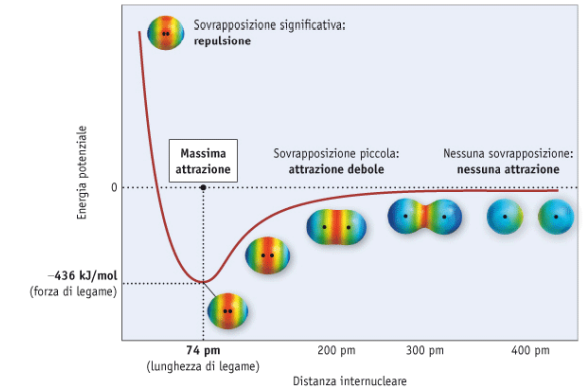
\includegraphics[width=12cm]{immagini/energia-potenziale.png}
\end{figure}

\vspace{-0.3cm}Essa sarà l'energia di due atomi di idrogeno che si avvicinano.

Inizialmente abbiamo valori di energia prossimi a zero, ossia quando la distanza è infinita questo sistema ha energia potenziale nulla. Nell'istante in cui la distanza diventa misurabile i due atomi iniziano ad interagire. Ciò significa che quando i due atomi si avvicinano si può già parlare di energia negativa e quindi i due atomi si stanno realmente legando, ossia possiamo immaginare che si inizi ad instaurare un legame chimico.

I due atomi si avvicineranno fino ad una certa distanza in cui si ha il minimo di energia per il sistema. Per due atomi di idrogeno legati tale minimo si ottiene quando la distanza di equilibrio (perché i due atomi vibrano, non sono rigidamente fermi) è pari 0.74 Å.

Se tentassimo di avvicinarli ulteriormente, l'energia inizierebbe a crescere velocemente superando persino lo zero, perché inizia ad essere incisiva la repulsione tra i nuclei e tra gli elettroni. Se invece li allontanassimo l'energia tenderebbe al valore U=0, che prende il nome di \textit{asintoto di dissociazione}, e i due atomi non sarebbbero più legati.

Nel punto di minimo in energia per due atomi di idrogeno si trova un valore di -436 kJ/mol, che è il valore di energia che dovremmo spendere per rompere il legame della molecola H$_2$.

\vspace{0.2cm}
Seguendo questa curva sembrerebbe che siano possibili tutte le energie, ma non è così. Infatti abbiamo detto che l'energia è quantizzata, e tale è anche l'energia di vibrazione di due atomi di idrogeno all'interno di una molecola di H$_2$, per cui solo alcuni dei valori rappresentati sono permessi. Questo modo di rappresentare l'energia è più adatto per un sistema macroscopico i cui valori di energia non siano quantizzati. Tuttavia si usa comunque questa rappresentazione per sistemi quantizzati, dato che i valori possibili di energia stanno su questa curva.

\vspace{-0.5cm}\begin{figure}[htp]
    \centering
    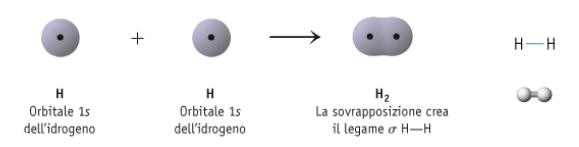
\includegraphics[width=12cm]{immagini/legame-H_2.png}
\end{figure}

\vspace{-0.5cm}Quello che quindi stiamo immaginando è di avere due atomi di idrogeno con due orbitali 1s, ciascuno con un proprio elettrone. Questi due orbitali interagiscono tra di loro per dar luogo alla formazione di un legame chimico, con l'ottenimento della molecola H$_2$. Se abbiamo due orbitali di tipo s, cioè a simmetria sferica, si ottiene un legame di tipo $\sigma$, che è quello che rappresentiamo come una lineetta tra i due atomi di idrogeno. 

\vspace{0.2cm}Consideriamo adesso l'acido fluoridrico HF. Il fluoro è il primo degli alogeni e ha orbitali 2s e 2p come orbitali di valenza. L'orbitale 2s è parecchio interno come energia, quindi non adatto per interagire con l'orbitale 1s dell'atomo di idrogeno. Abbiamo poi i tre orbitali p: uno di questi avrà i suoi lobi orientati lungo quello che etichettiamo \textit{asse di legame}. L'orbitale p del fluoro orientato lungo tale asse, interagirà con l'orbitale 1s dell'idrogeno e formerà un legame $\sigma$, perché si ha sovrapposizione lungo l'asse di legame, sebbene gli orbitali interagenti siano uno di tipo s e uno di tipo p.

\vspace{-0.5cm}\begin{figure}[htp]
    \centering
    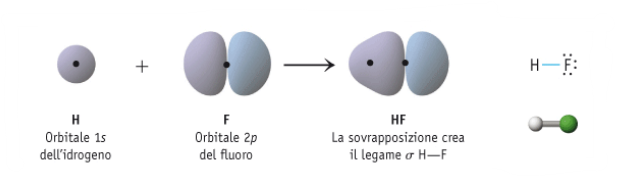
\includegraphics[width=12cm]{immagini/legame_H-F.png}
\end{figure}

\vspace{-0.5cm}Va da notare che i due lobi dell'orbitale p hanno colori diversi, e ad interagire con l'orbitale s dell'idrogeno è quello che ha lo stesso colore di ques'ultimo. Il motivo è che i lobi degli orbitali p hanno segno opposto, pertanto affinché i due orbitali interagiscano si deve scegliere il lobo avente lo stesso segno dell's.

\vspace{0.2cm} Prendiamo adesso in esame la molecola F$_2$. Essendo due atomi identici, essi avranno gli stessi orbitali, e in particolare quelli più esterni nel fluoro sono i p. Per ciascun atomo di fluoro, uno dei tre giacerà lungo l'asse di legame:

\vspace{-0.5cm}\begin{figure}[htp]
    \centering
    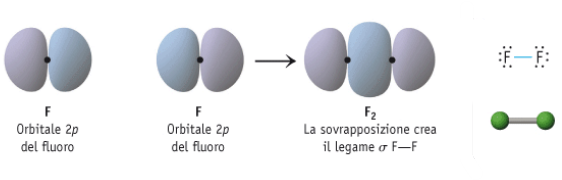
\includegraphics[width=10cm]{immagini/legame-F_2.png}
\end{figure}

\vspace{-0.5cm}Se li orientiamo in modo tale che i lobi che si affacciano l'uno sull'altro abbiano lo stesso segno, ancora una volta otterremo un orbitale $\sigma$, in quanto ci sarà addensamento lungo la congiungente i due nuclei cioè lungo l'asse di legame, nonostante esso si stia formando tramite due orbitali p.

\vspace{0.2cm} Da questi esempi deduciamo che il legame $\sigma$ non necessariamente debba venir fuori da due orbitali di tipo s, ma può venir fuori anche un orbitale s e uno p o da due orbitali p. La cosa fondamentale è che gli orbitali che interagiscono siano orientati lungo la stessa direzione.
\subsection{Gli orbitali molecolari}
La teoria degli orbitali molecolari considera la molecola come un insieme di nuclei e di elettroni e,
valutando le loro reciproche interazioni, determina le funzioni d’onda che descrivono gli elettroni nella
molecola in modo analogo a quello usato per individuare le funzioni d’onda che descrivono gli elettroni
negli atomi isolati.

\vspace{0.2cm}Consideriamo la molecola più semplice che esista: la molecola H$_2^+$. Il motivo per cui consideriamo lo ione piuttosto che la molecola H$_2$ è che questa è composta da due atomi di idrogeno, ognuno dei quali porta un elettrone, per cui nel complesso avremo due protoni e due elettroni, mentre nello ione abbiamo un solo elettrone. Tale fatto ci permette di studiarla tramite l'equazione di Schrödinger, per cui siamo in grado di ottenere le soluzioni esatte delle sue energie.

In termini semplici, l'atomo di idrogeno consiste di un protone e un elettrone. Nell'istante in cui abbiamo due protoni, quali energie bisogna considerare?

\hspace{1.5cm}\begin{minipage}{0.5\textwidth}
    \begin{figure}[H]
        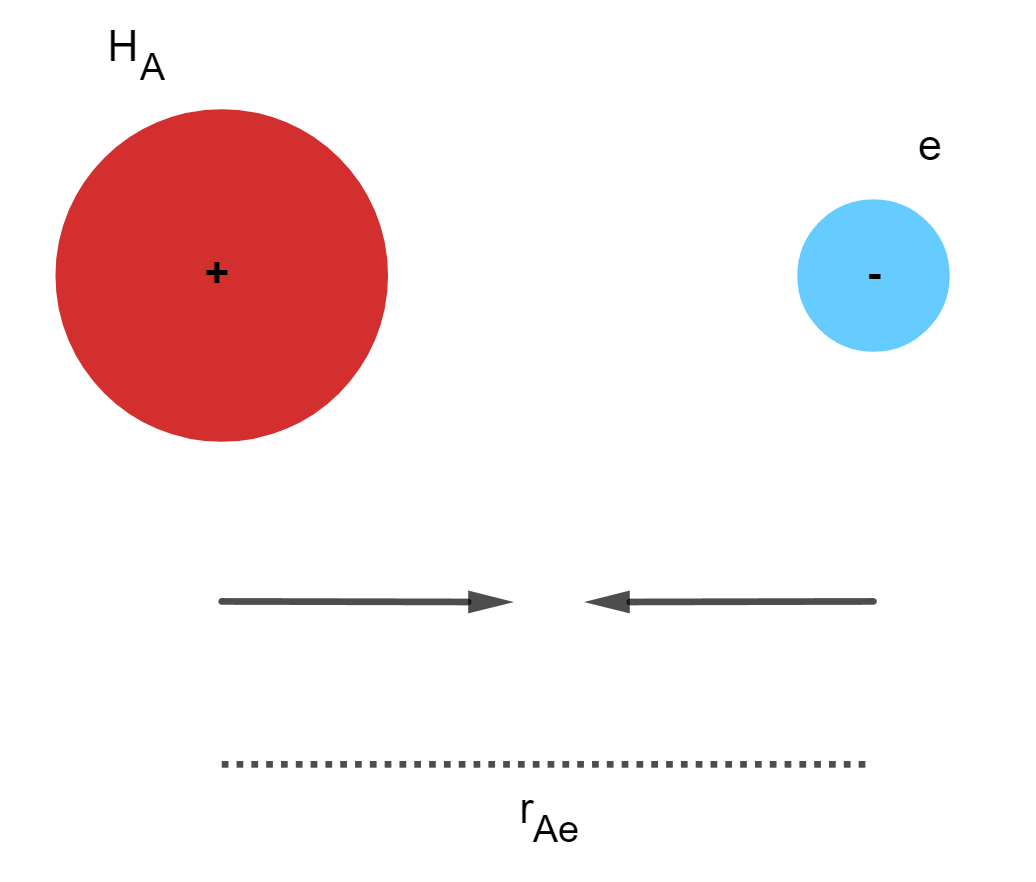
\includegraphics[width=4cm]{immagini/attrazione protone-elettrone.png}
    \end{figure}
    \end{minipage} \hfill
    \begin{minipage}{0.5\textwidth}
    \begin{figure}[H]
        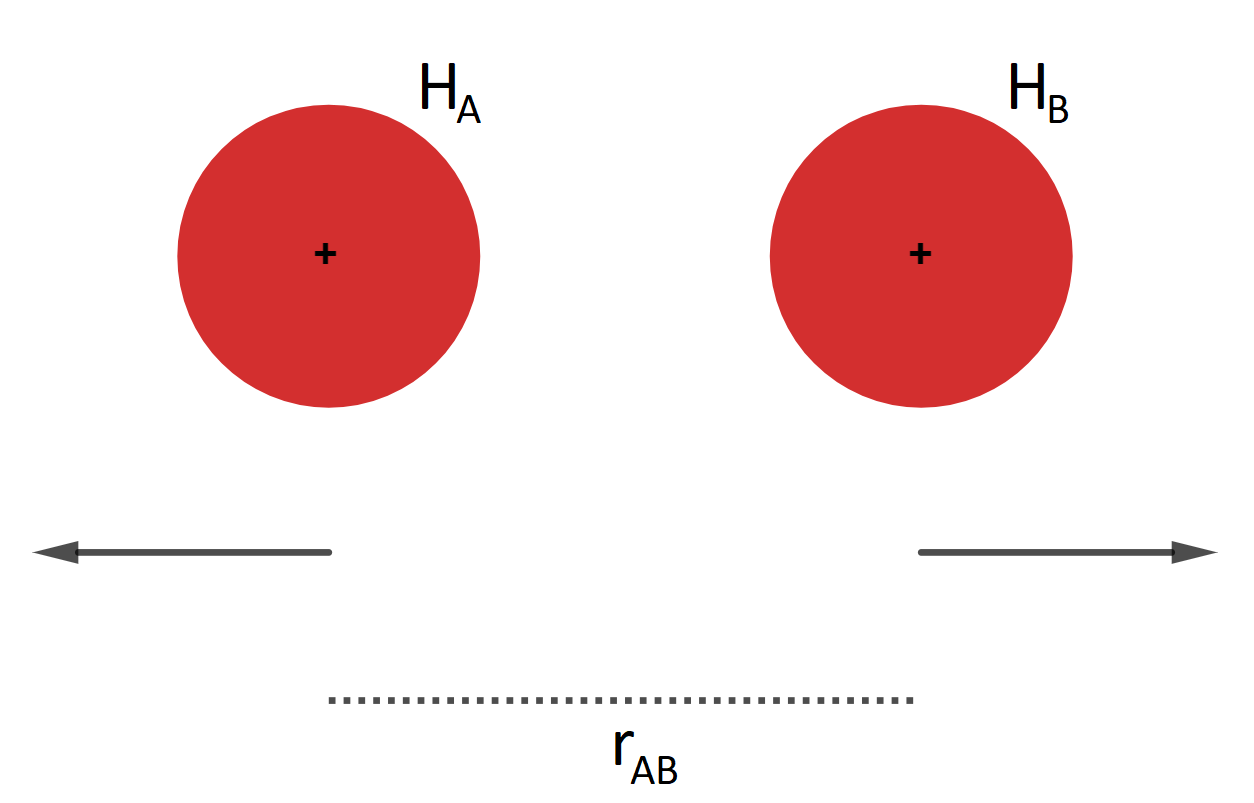
\includegraphics[width=5cm]{immagini/repulsione protone-protone.png}
    \end{figure}
    \end{minipage}

\comment{
    \begin{figure}[htp]
    \centering
    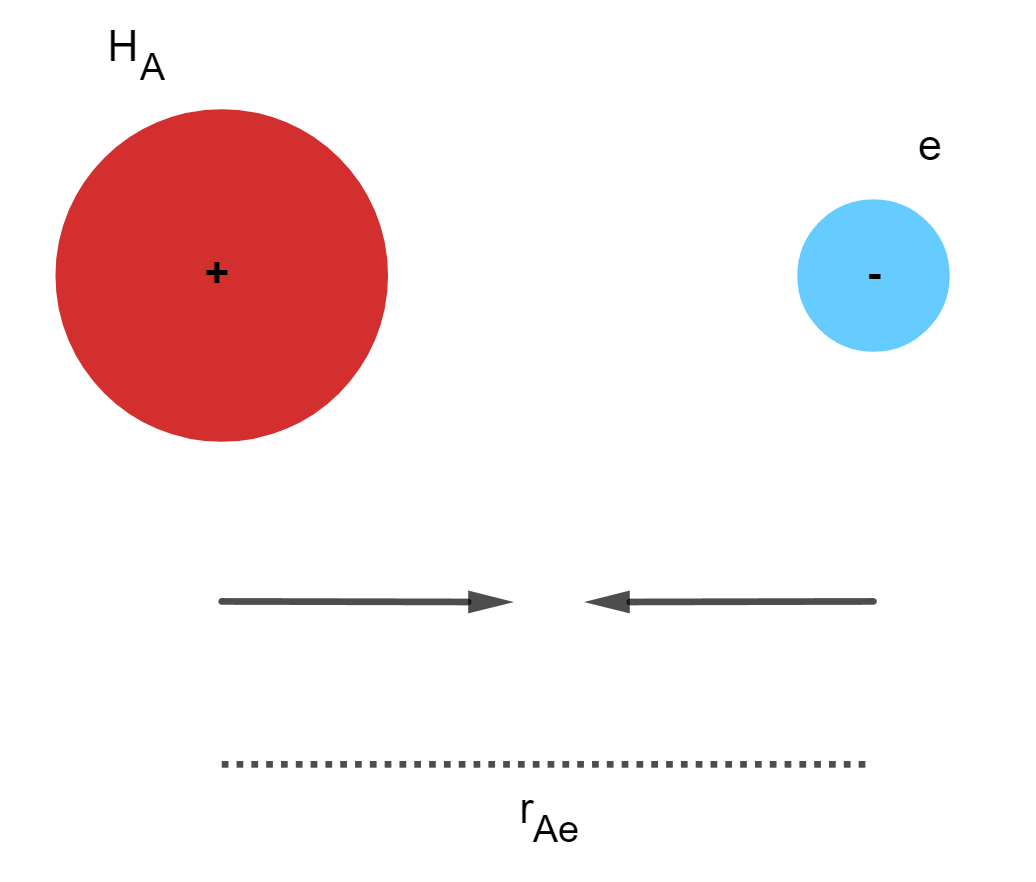
\includegraphics[width=4cm]{immagini/attrazione protone-elettrone.png}
\end{figure}
}
Una prima energia sarà data dall'attrazione tra l'elettrone e il nucleo dell'atomo di idrogeno A. Esso vale $E=-\frac{q^2}{r_{Ae}}$, ed essendo negativo abbassa l'energia del sistema.

Un secondo contributo analogo si avrà dall'attrazione tra l'elettrone e l'atomo di idrogeno B: $E=-\frac{q^2}{r_{Be}}$

Un terzo e ultimo contributo sarà dato dalla repulsione tra i due nuclei. Tale energia vale $E=\frac{q^2}{r_{AB}}$, ed essendo positivo alzerà l'energia.

\vspace{0.2cm}L'elettrone quindi interagisce con entrambi i nuclei:
\begin{figure}[htp]
    \centering
    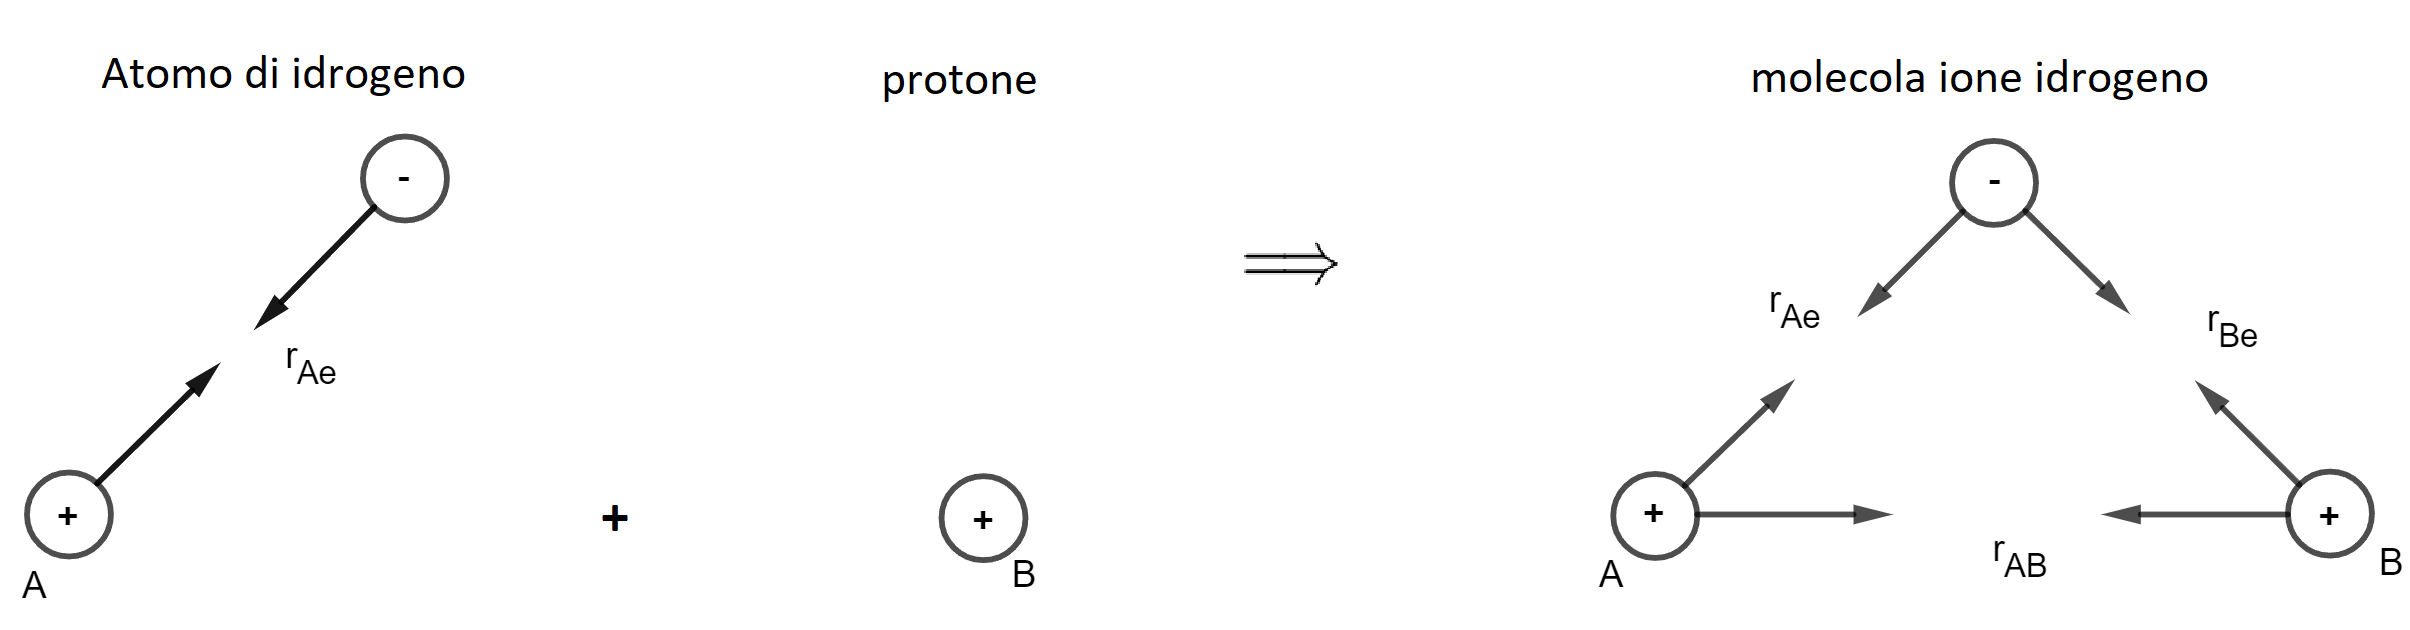
\includegraphics[width=14cm]{immagini/interazione_elettrone_con_protoni.png}
\end{figure}

Avremo tre distanze: quella tra il nucleo A e l'elettrone $r_{Ae}$, quella tra il nucleo B e l'elettrone $r_{Be}$ e quella tra i due nuclei $r_{AB}$.

Va da ricordare che la meccanica quantistica studia stati stazionari, cioè indipendenti dal tempo, il che significa che stiamo immaginando la molecola come se fosse rigida, cioè nel momento in cui andiamo a fare questi calcoli immaginiamo che non esistano vibrazioni ecc.

I termini energetici che avremo sono:
$$\ce{H_A^+-H_B^+ \quad + \quad H_A^+-e^- \quad + \quad H_B^+-e^-}$$
$$\text{repulsione \qquad attrazione \qquad attrazione}$$
$$\frac{q^2}{r_{AB}} \qquad - \qquad \frac{q^2}{r_{Ae}} \qquad - \qquad \frac{q^2}{r_{Be}}$$

Se immmaginiamo di avere particelle in posizioni fissate, possiamo andare a vedere qual è la composizione delle forze.

\begin{figure}[htp]
    \centering
    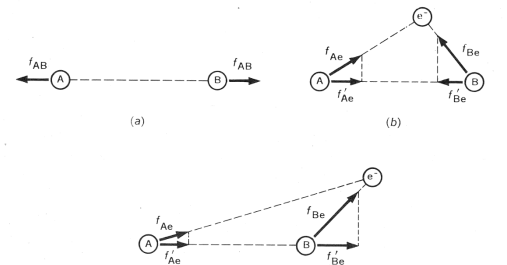
\includegraphics[width=11cm]{immagini/posizone_elettrone.png}
\end{figure}

Si nota che se questo elettrone, anziché essere fra i due nuclei fosse in una regione diversa (ad esempio a destra del nucleo B) sentirebbe l'attrazione di un nucleo, ma non è detto che senta quella dell'altro.

Quindi formalmente se l'elettrone viene immaginato come una particella, è chiaro che la sua posizione nello spazio è importante.

Secondo la teoria degli orbitali molecolari, quando si formano molecole il numero di orbitali che ogni atomo possiede contribuirà agli orbitali molecolari che troveremo sulla molecola. Questo significa che se un atomo ha n orbitali di valenza, tutti questi contribuiranno a formare un ugual numero di orbitali molecolari.

In questo esempio abbiamo un orbitale 1s su ciascun atomo di idrogeno, per cui otterremo due orbitali molecolari: avremo una combinazione detta \textbf{in fase} delle funzioni d'onda 1s$_A$ + 1s$_B$, e una combinazione detta \textbf{fuori fase} delle funzioni d'onda 1s$_A$ - 1s$_B$. La prima è detta \textbf{combinazione di legame}, la seconda di \textbf{antilegame}. In termini spaziali significa che per una data molecola lo spazio si divide in due regioni che daranno luogo, se è lì presente l'elettrone, alla combinazione legante e a quella antilegante:

\begin{figure}[htp]
    \centering
    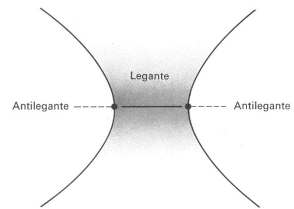
\includegraphics[width=6cm]{immagini/spazio_legante_antilegante.png}
\end{figure}

L'orbitale di antilegame si chiama così perché riempirlo non dà forza, anzi tende a distruggere il legame, a differenza di quello di legame che se riempito rafforza il legame.

Deduciamo che di volta in volta dovremo fare i conti, in modo da capire quanti sono gli orbitali interagenti e quanti elettroni abbiamo a disposizione, in quanto le proprietà del legame dipenderanno da quanti orbitali di legame e quanti di antilegame si riempiranno.

\vspace{0.2cm}Sappiamo che sovrapporre due orbitali atomici di tipo s significa ottenere orbitali molecolari di tipo $\sigma$. Supponiamo di avere due atomi di idrogeno distanti. Man mano che li avviciniamo, anche i loro orbitali atomici si avvicineranno, fino a sovrapporsi. Se ricordiamo l'andamento dell'energia potenziale, essa ha un minimo ad una distanza ben precisa sopra e sotto la quale l'energia è maggiore:

\begin{figure}[htp]
    \centering
    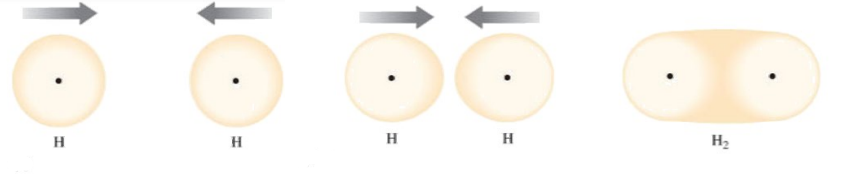
\includegraphics[width=12cm]{immagini/avvicinamento_orbitali.png}
\end{figure}

Supponiamo di essere alla distanza esatta che produce un minimo di energia. Essendoci un addensamento lungo la congiungente i nuclei ovvero lungo l'asse di legame, si ha un'interazione di tipo $\sigma$.

\vspace{0.2cm}Anche un orbitale s con un orbitale p, e persino due orbitali p orientati entrambi lungo l'asse di legame, danno luogo a un'interazione $\sigma$ che produce due orbitali: uno di legame  $\sigma$ e uno di antilegame  $\sigma^*$.

\hspace{1cm}\begin{minipage}{0.36\textwidth}
    \begin{figure}[H]
        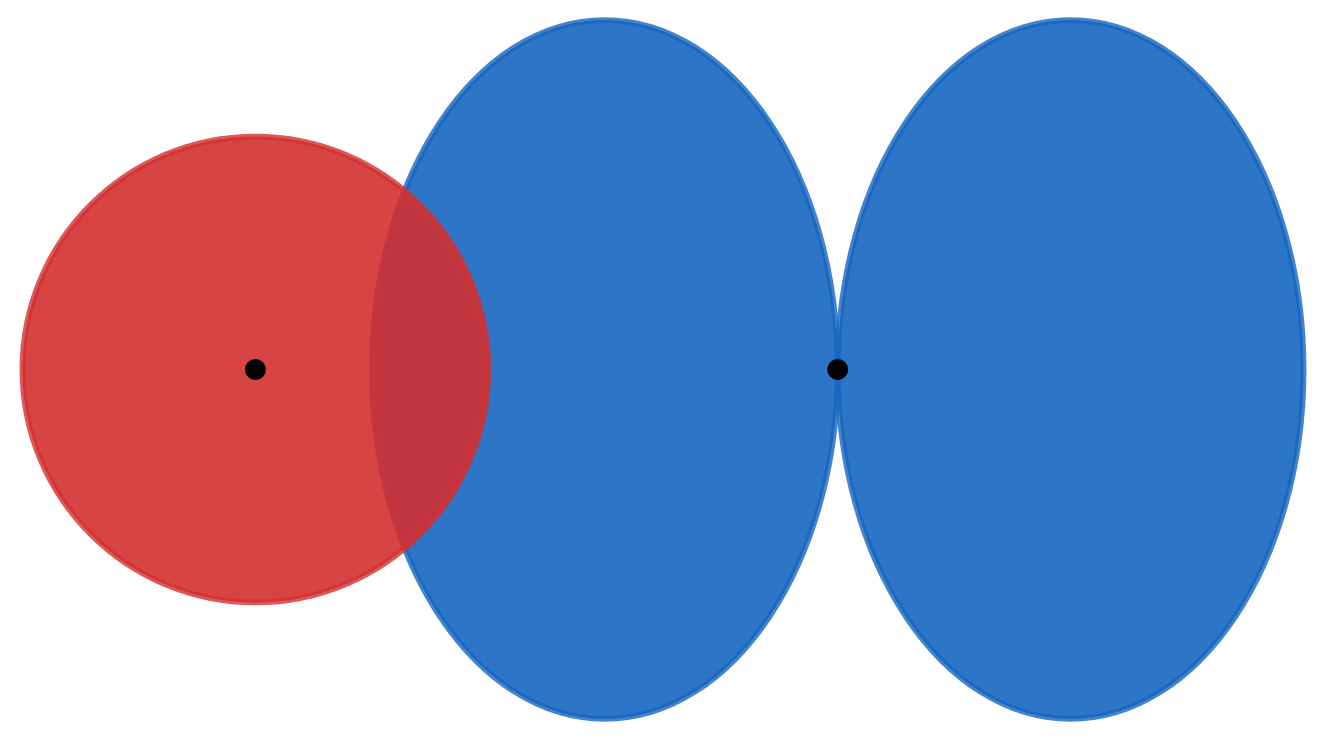
\includegraphics[width=4cm]{immagini/legame_sigma_s_p.png}
    \end{figure}
    \end{minipage} 
\begin{minipage}{0.4\textwidth}
    \vspace{-0.5cm}\begin{figure}[H]
        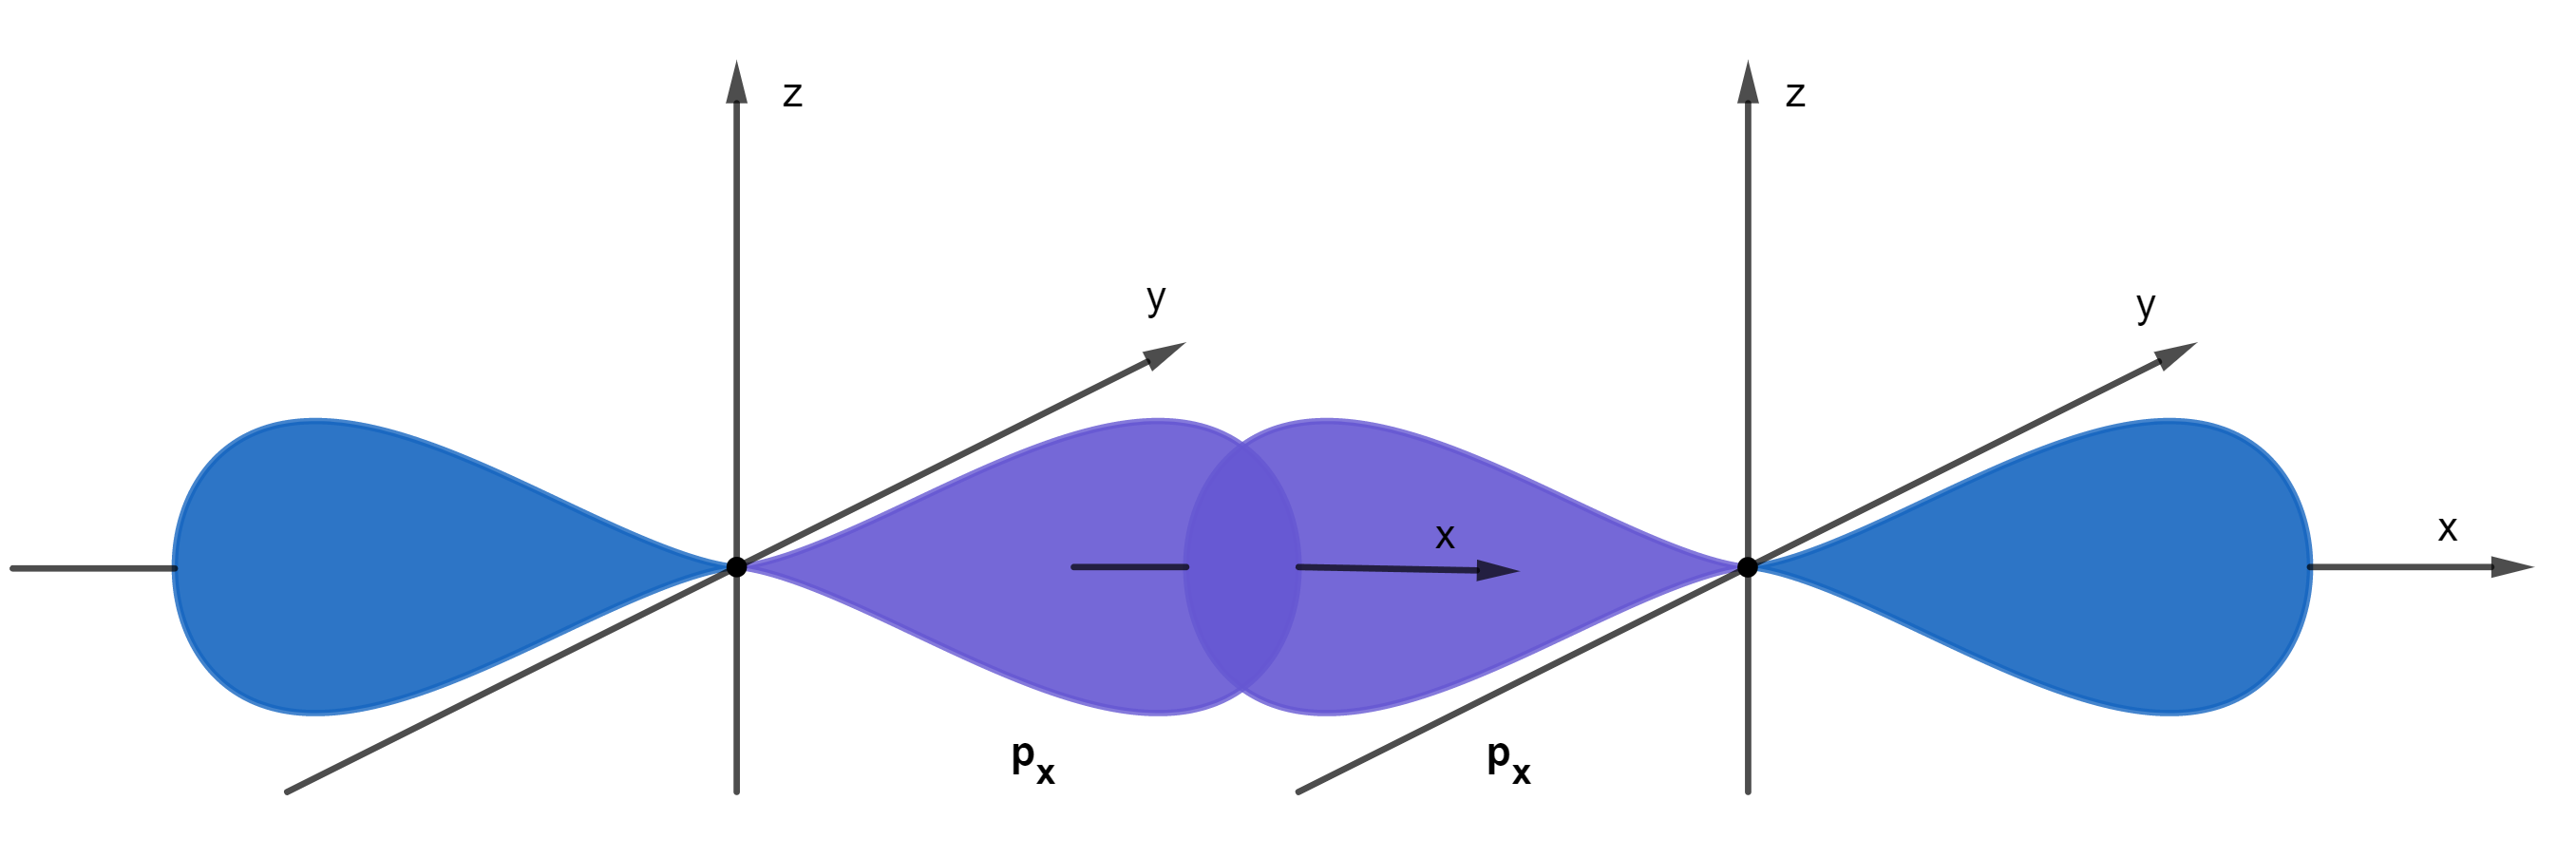
\includegraphics[width=8cm]{immagini/legame_sigma_p_p.png}
    \end{figure}
    \end{minipage}

\vspace{0.2cm}(Nel grafico è riportata solo la combinazione di legame).

L'orbitale molecolare di legame sarà quello nel quale i lobi degli orbitali atomici interagenti (cioè le funzioni d'onda) hanno lo stesso segno, mentre in quello di antilegame hanno segno opposto.

Nel caso di interazione $\sigma$ tra due orbitali p, se abbiamo stabilito (come nel caso del grafico) che questi siano orientati lungo l'asse $x$, gli orbitali p$_y$ e p$_z$ saranno perpendicolari a tale asse e daranno lugo a sovrapposizioni $\pi$:

\hspace{1cm}\begin{minipage}{0.5\textwidth}
    \begin{figure}[H]
        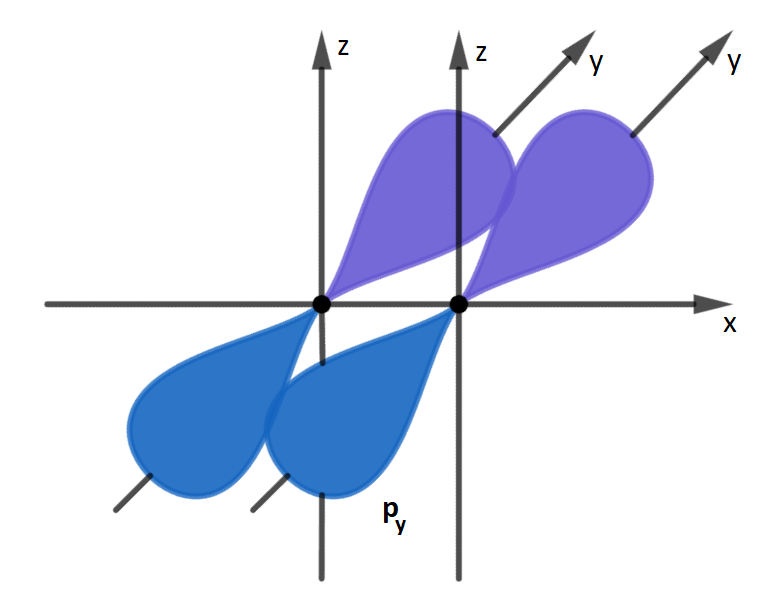
\includegraphics[width=6cm]{immagini/orbitali_py.png}
    \end{figure}
    \end{minipage} \hfill
    \begin{minipage}{0.5\textwidth}
    \begin{figure}[H]
        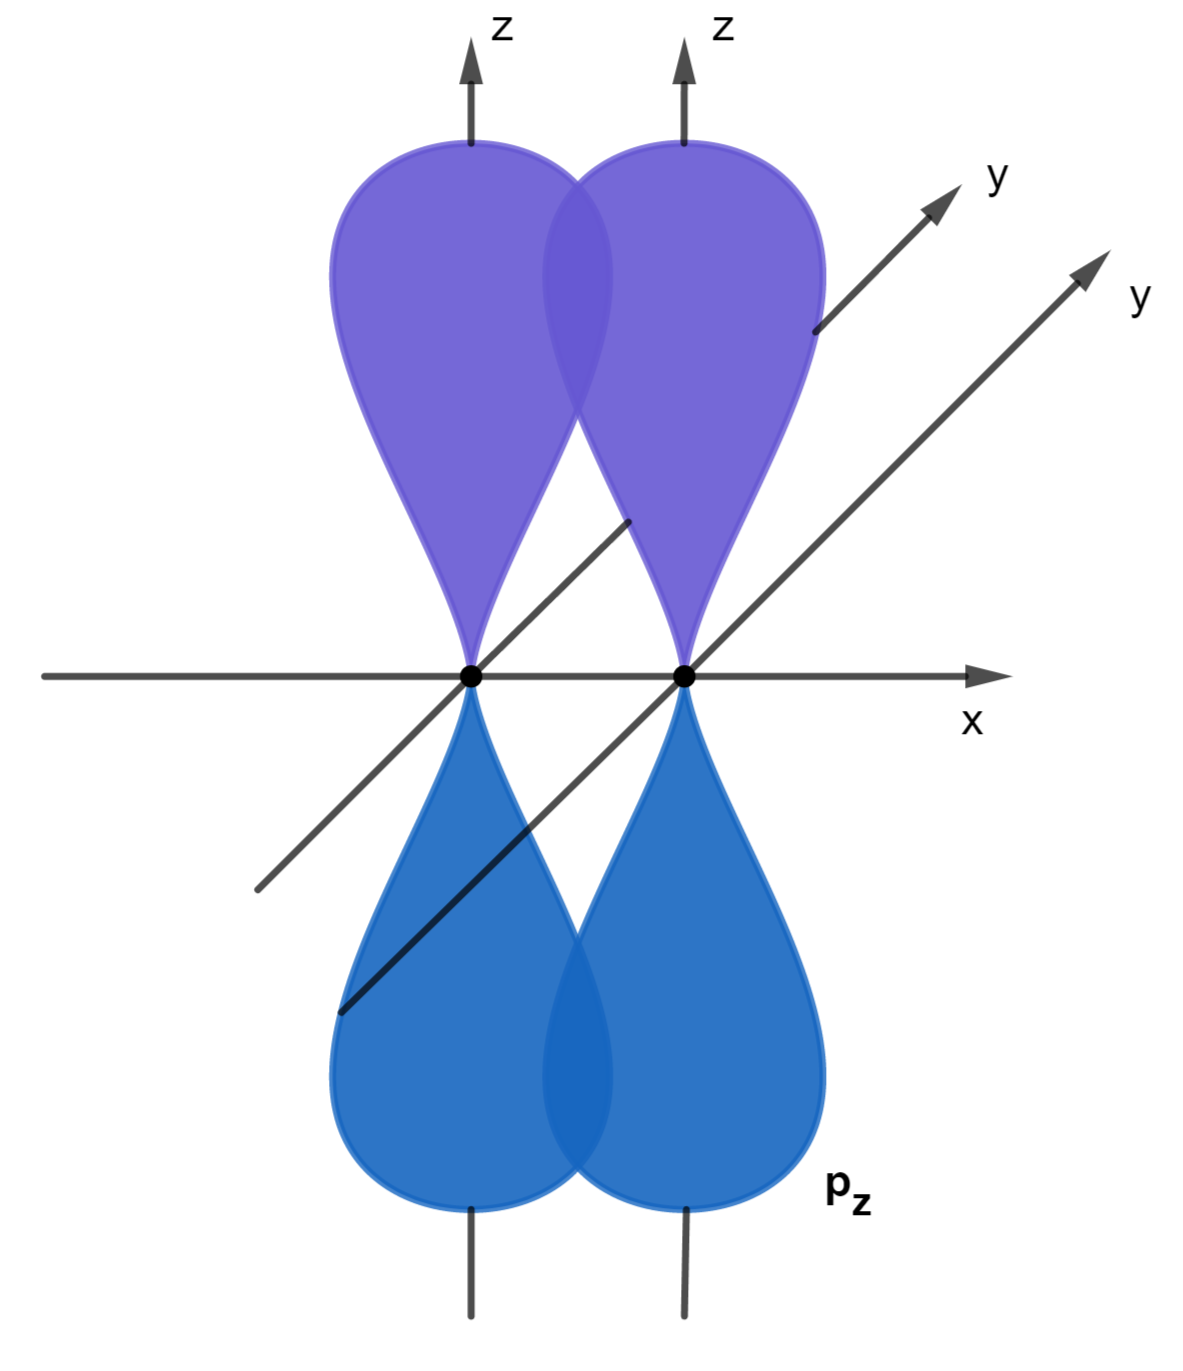
\includegraphics[width=4cm]{immagini/orbitali_pz.png}
    \end{figure}
    \end{minipage}

Quindi per una coppia di orbitali p avremo una sovrapposizione diretta lungo la congiungente i due nuclei, mentre per le altre due coppie la sovrapposizione avverrà sopra e sotto.

\vspace{0.2cm}Consideriamo adesso le forze attrattive e repulsive nel legame covalente:

\begin{figure}[H]
    \centering
    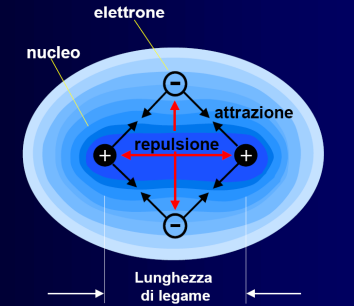
\includegraphics[width=7cm]{immagini/forze_legame_covalente.png}
\end{figure}
 
Questo è il modello che dobbiamo considerare quando studiamo composti nei quali il legame è covalente. In questo caso non stiamo parlando di cessione di elettroni, come invece se ne parla nel legame ionico.

Se abbiamo due nuclei di idrogeno e due elettroni, questi ultimi daranno luogo a forze attrattive in certe posizioni rispetto ad altre.

\vspace{0.2cm}Riguardiamo la formazione della molecola H$_2$:

\begin{figure}[H]
    \centering
    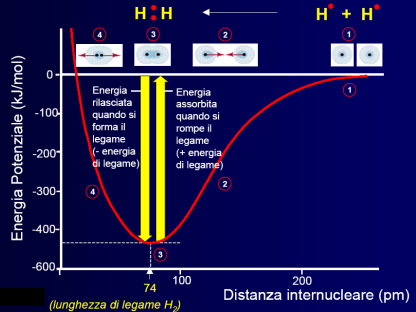
\includegraphics[width=11cm]{immagini/legame_covalente_H_2.png}
\end{figure}

Due atomi di idrogeno inizialmente molto distanti hanno energia potenziale praticamente nulla, ossia non interagiscono. Iniziamo ad avvicinare i due atomi e l'energia potenziale si abbassa. Appena li avviciniamo fino a 0.74 Å raggiungiamo il minimo. Si sono così formati i due orbitali molecolari, uno di legame e uno di antilegame. Se avvicinassimo i due atomi ancora di più, l'energia potenziale tornerebbe a crescere a causa delle interazioni repulsive tra i nuclei e tra gli elettroni, i quali si troverebbero a occupare la stessa piccola regione di spazio. Quindi la distanza intermolecolare è importante al fine di capire se questo sistema ha raggiunto il minimo di energia.

Va da ricordare che per il sistema non sono possibili tutte le energie, ma solo alcuni valori quantizzati di questa.
\subsection{Orbitali molecolari leganti ed antileganti $\boldsymbol{\sigma}$}

Ragioniamo ancora sulla molecola H$_2$.

Abbiamo due orbitali atomici, che chiameremo 1s(A) e 1s(B). Quando combiniamo le funzioni d'onda con lo stesso segno, avremo la combinazione \textit{in fase} o \textit{legante}, la cui funzione d'onda è data da una combinazione lineare delle funzioni d'onda atomiche:
$$\Psi(VB)=\Psi\text{(1s)A} + \Psi\text{(1s)B} \quad \text{(combinazione legante)}$$
Se invece i due orbitali 1s interagissero con funzioni d'onda il cui segno è opposto, avremo la combinazione \textit{fuori fase} o \textit{antilegante}:
$$\Psi^*(VB)=\Psi\text{(1s)A} - \Psi\text{(1s)B} \quad \text{(combinazione antilegante)}$$

Tracciamo una scala energetica:

\begin{figure}[htp]
    \centering
    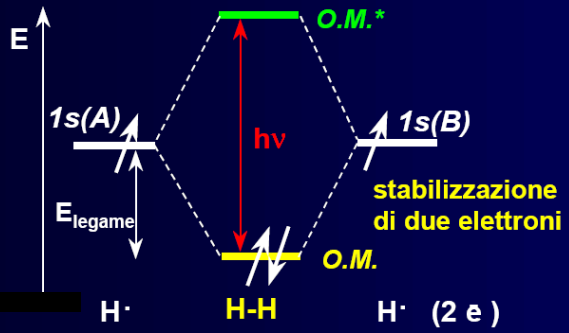
\includegraphics[width=9cm]{immagini/scala_energia_H_2.png}
\end{figure}

In questa scala qualitativa, abbiamo due orbitali di due atomi identici, quindi li mettiamo a pari livello. La freccia $\nearrow$ sta a indicare la presenza di un elettrone su ciascun orbitale.

Si avrà una interazione in fase con abbassamento di energia e una fuori fase con innalzamento in energia.

\begin{figure}[htp]
    \centering
    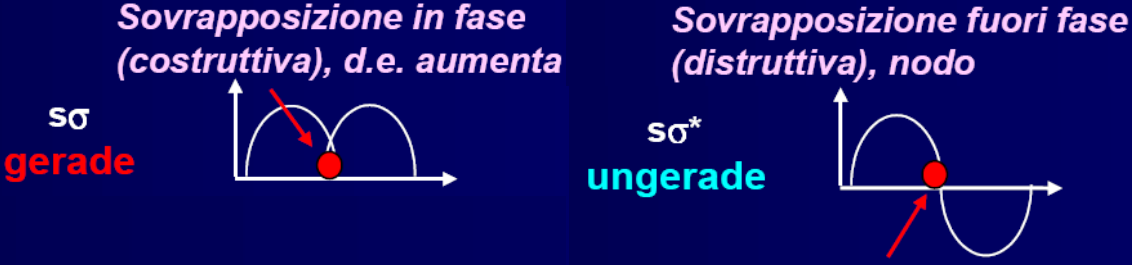
\includegraphics[width=12cm]{immagini/sovrapposizione_in_fase_e_fuori_fase.png}
\end{figure}

La funzione d'onda molecolare dell'orbitale legante mostra addensamento lungo la congiungente i nuclei, quella dell'orbitale antilegante mostra un nodo lungo essa.

\vspace{0.2cm}Dato che abbiamo solo due elettroni, entrambi andranno a riempire il livello più basso in energia. Quindi avremo una stabilizzazione netta di questi due elettroni, i quali prima si trovavano a un livello energetico più alto negli orbitali 1s, mentre adesso si trovano a energia più bassa perché la combinazione in fase si è stabilizzata. Lasciamo invece vuoto l'orbitale molecolare di antilegame.

La molecola allora si forma perché c'è una stabilizzazione netta di questi due elettroni, che passano da una energia più alta ad una più basse.

Va da ricordare che quando si hanno queste interazioni verrà sepre mantenuto il baricentro di energia, ciò significa che la differenza di energia tra il livello di partenza e l'orbitale molecolare di legame sarà uguale alla differenza di energia tra il livello di partenza e l'orbitale molecolare di antilegame, ossia da un punto di vista energetico la stabilizzazione sarà uguale alla destabilizzazione, cioè le due quantità sono uguali.

La molecola H$_2$ quindi esiste solo perché nei fatti i due elettroni dei due atomi di idrogeno interagenti andranno a occupare il livello più basso in energia, avendo quindi un guadagno netto da un punto di vista energetico.

\subsection{L'ordine di legame (O.L.)}
Adesso possiamo esplicitare meglio il concetto di ordine di legame.

Esso va caclolato così:
$$\text{O.L.}=\frac{\text{n° di elettroni leganti - n° di elettroni antileganti}}{2}$$
dove gli elettroni leganti sono gli elettroni presenti negli orbitali di legame e quelli antileganti sono quelli presenti negli orbitali di antilegame.

Nel caso della molecola H$_2$ abbiamo 2 elettroni negli orbitali di legame e 0 elettroni in quelli di antilegame, per cui
$$\text{O.L.}=\frac{2-0}{2}=1$$

Essendo l'ordine di legame pari a 1, questa molecola si scrive con un legame semplice.

\vspace{0.2cm}Immaginiamo di avere due atomi di idrogeno A e B. La rappresentazione grafica delle loro funzioni d'onda è

\begin{figure}[H]
    \centering
    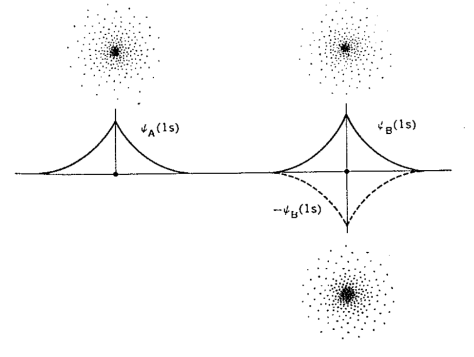
\includegraphics[width=10cm]{immagini/orbitali_atomici.png}
\end{figure}

Immaginiamo quindi di avvicinare i due nuclei, sia nel caso della combinazione in fase che in quello della combinazione fuori fase:

\begin{figure}[H]
    \centering
    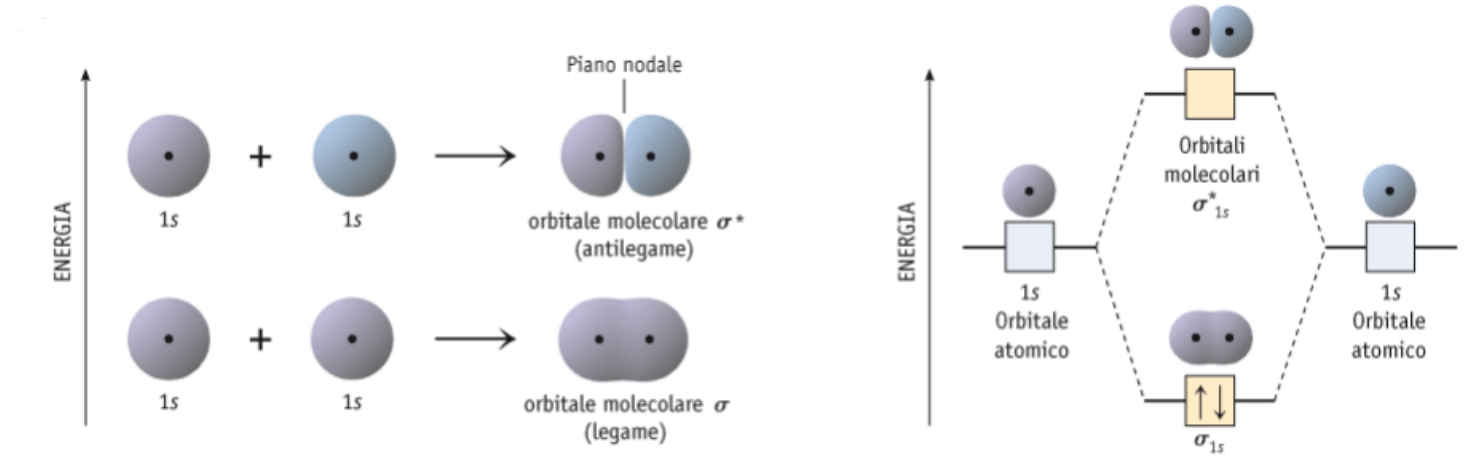
\includegraphics[width=16cm]{immagini/orbitali_molecolari_H_2.png}
\end{figure}

Se combiniamo due orbitali 1s con lo stesso segno di due atomi di idrogeno otterremo un orbitale molecolare di legame (di tipo $\sigma$ perché il legame avviene lungo la congiungente i nuclei).

Se combiniamo due orbitali 1s con segni diversi otteniamo un orbitale molecolare di antilegame (di tipo $\sigma^*$), infatti abbiamo un nodo lungo l'asse di legame.

\begin{figure}[htp]
    \centering
    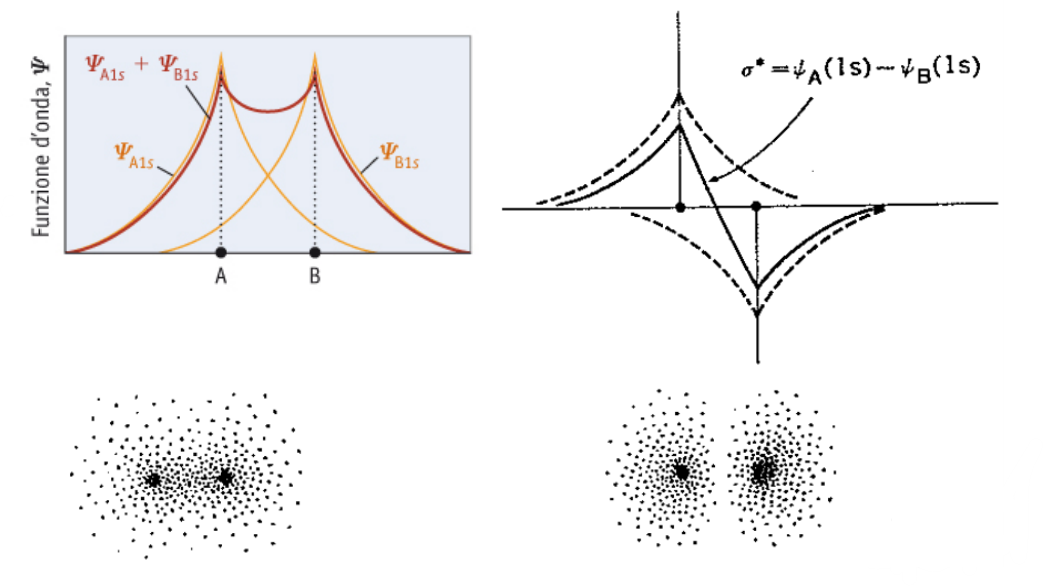
\includegraphics[width=12cm]{immagini/combinazione_funzioni.png}
\end{figure}

Possiamo quindi combinare sia due parti entrambe positive che una parte positiva e una negativa.

Nel primo caso quello che succede è che avvicinando i nuclei avremo una zona in comune, per cui la funzione si alza, cioè lungo la congiungente i nuclei, nell'orbitale $\sigma$ di legame, si avrà la funzione che cresce.

Al contrario, nell'altro caso, esattamente al centro tra i due nuclei la funzione si annulla (ci sarà un piano nodale).

Si ha quindi, ricapitolando, sovrapposizione di orbitali che rappresentiamo con la funzione d'onda e, a seconda che si abbia combinazione in fase o fuori fase, aumenterà l'ampiezza della funzione d'onda tra i due nuclei o viceversa diventerà zero.

Dunque avremo sempre una combinazione in fase che darà luogo ad un orbitale $\sigma$ e una fuori fase che darà luogo a un orbitale $\sigma^*$. Dopodiché aggiungeremo gli elettroni, che nel caso della molecola H$_2$ occupano esclusivamente l'orbitale molecolare di legame.

Quindi sostanzialmente rispetto ad un valore di energia che possiamo immaginare essere il punto di riferimento (ossia l'energia degli orbitali non interagenti), avremo un abbassamento in energia della combinazione in fase e un innalzamento in energia della combinazione fuori fase.

\vspace{0.2cm}Iniziamo allora a vedere quanti elettroni riusciamo a sistemare in questo sistema costituito da due orbitali atomici interagenti che formano due orbitali molecolari:

\vspace{0.2cm}\hspace{1.5cm}\begin{minipage}{0.1\textwidth}
    \begin{figure}[H]
        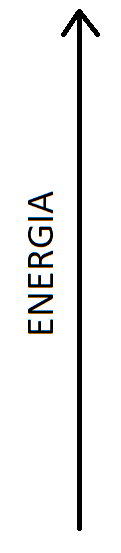
\includegraphics[width=1cm]{immagini/freccia_energia.png}
    \end{figure}
\end{minipage} \hfill
\begin{minipage}{0.95\textwidth}
        \begin{tabular}{m{4cm}|m{1.5cm}m{1.5cm}m{1.5cm}m{1.5cm}}
            \vspace{0.4cm}& \ce{H_2^+} & \ce{H_2} & \ce{He_2^+} & \ce{He_2}\\
            \vspace{0.4cm}$\boldsymbol{\sigma^*}(1s)$ & \vspace{0.4cm}\orbital{0} & \vspace{0.4cm}\orbital{0} & \vspace{0.4cm}\orbital{1} & \vspace{0.4cm}\orbital{2}\\
            \\
            \vspace{0.4cm}$\boldsymbol{\sigma}(1s)$ & \vspace{0.4cm}\orbital{1} & \vspace{0.4cm}\orbital{2} & \vspace{0.4cm}\orbital{2} & \vspace{0.4cm}\orbital{2}\\
            \vspace{0.4cm}Numero di elettroni & \vspace{0.4cm}\hspace{0.1cm}1 & \vspace{0.4cm}\hspace{0.1cm}2 & \vspace{0.4cm}\hspace{0.1cm}3 & \vspace{0.4cm}\hspace{0.1cm}4\\
            \vspace{0.2cm}Ordine di legame & \vspace{0.2cm}\hspace{0.05cm}$\displaystyle\frac{1}{2}$ & \vspace{0.2cm}\hspace{0.1cm}1 & \vspace{0.2cm}\hspace{0.05cm}$\displaystyle\frac{1}{2}$ & \vspace{0.2cm}\hspace{0.1cm}0
        \end{tabular}
\end{minipage}

\vspace{0.2cm}$\bullet$Esiste la molecola \ce{H_2^+}, avente due atomi di idrogeno e un solo elettrone, il quale andrà nell'orbitale a più bassa energia. Questa è inferiore rispetto all'energia del sistema di riferimento, quindi questa molecola deve esistere. Il suo ordine di legame è 1/2;

\vspace{0.2cm}$\bullet$ Con la molecola H$_2$ riempiamo totalmente il livello più basso in energia con due elettroni. L'ordine di legame sarà 1, quindi per rappresentare questa molecola mettiamo un legame semplice;

\vspace{0.2cm}$\bullet$ L'elio è l'elemento successivo all'idrogeno, quindi ha due elettroni, ma l'orbitale continua a essere l'1s, per cui nella molecola He$_2$ si genera ancora un orbitale $\sigma$ e uno $\sigma^*$. Stavolta però avremo in totale quattro elettroni, il che significa che riempiamo totalmente sia l'orbitale di legame che quello di antilegame. Da ciò capiamo che non ci sarà alcun guadagno in energia rispetto alla situazione dei due atomi non interagenti, perché avendo mantenuto il baricentro di energia l'energia guadagnata riempiendo totalmente l'orbitale di legame è uguale a quella persa riempiendo totalmente l'orbitale di antilegame.

L'ordine di legame allora sarà pari a zero. il che significa che questa molecola non puà esistere, e nei fatti l'elio non esiste in forma molecolare;

\vspace{0.2cm}$\bullet$ Supponiamo per assurdo che l'He$_2$ esista e strappiamogli un elettrone: otterremo la specie He$_2^+$, avente tre elettroni. Due di questi riempiranno l'orbitale molecolare di legame e solo uno riempirà parzialmente quello di antilegame. Siccome due elettroni si stabilizzano e solo uno si destabilizza, si avrà un guadagno in energia. Infatti anche l'ordine di legame risulta diverso da zero: esso è pari a 1/2.

In questo modo dimostriamo che non può esistere la molecola He$_2$, ma esiste il suo catione He$_2^+$.

\vspace{0.2cm} Ciò che stiamo studiando è l'esito di una trattazione quanto-meccanica, e per questi sistemi il modello che ci propone la meccanica quantistica è perfetto, perché nei fatti ci permette di razionalizzare l'esistenza o meno di alcune molecole.

\vspace{0.2cm}Consideriamo adesso il litio, che è un metallo.

Immaginiamo la molecola fatta da due atomi di litio. Può esistere questa molecola?

Consideriamo gli orbitali coinvolti, i quali non sono tutti quelli di valenza, perché se abbiamo l'orbitale 2s dobbiamo avere anche gli orbitali 2p, in quanto avendo il numero quantico principale pari a 2, l può valere 0 (orbitali s) o 1 (orbitali p). Tuttavia non abbiamo elettroni a sufficienza per riempire i livelli 2p, quindi non li rappresenteremo:

\begin{figure}[H]
    \centering
    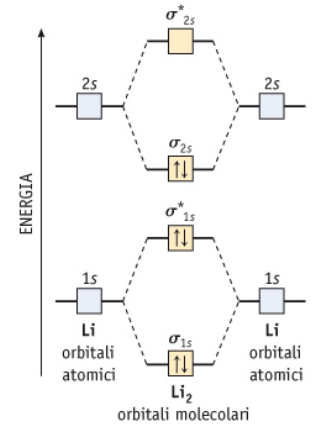
\includegraphics[width=10cm]{immagini/orbitali_molecolari_Li_2.png}
\end{figure}

Abbiamo gli orbitali 1s totalmente pieni perché nel litio l'1s è pieno con due elettroni, quindi in totale ne avremo quattro. Avremo poi la combinazione in fase e quella fuorifase dei due livelli 1s. Dunque abbiamo due orbitali molecolari con quattro elettroni, quindi riempiamo totalmente sia l'orbitale $\sigma_{1s}$ che quello $\sigma^*_{1s}$, pertanto questi elettroni non contribuiranno all'ordine di legame (2-2=0), ossia questi livelli non contribuiscono al legame chimico nella molecola Li$_2$.

\vspace{0.2cm}Andiamo adesso all'orbitale 2s. Va da ricordare che il litio sta sotto l'idrogeno, per cui la sua configurazione elettronica esterna è $\rm 2s^1$, cioè un solo elettrone.
    
Quello che vale per gli $1s$ vale anche per i $2s$, quindi avremo un'altra combinazione in fase $\sigma_{2s}$ e una fuorifase $\sigma_{2s}^*$. Abbiamo solo due elettroni in totale, i quali andranno ad occupare il livello più basso in energia, cioè l'orbitale $\sigma_{2s}$, lasciando vuoto il $\sigma_{2s}^*$. Già da ciò capiamo che questa molecola ha una sua stabilità.

\vspace{0.2cm}Se andiamo a calcolare l'ordine di legame avremo (4-2)/2=1: la molecola Li$_2$ esiste e va scritta con un legame semplice \ce{Li-Li}.

\vspace{0.2cm}Va da notare che non era nemmeno necessario rappresentare i livelli 1s perché sono a numero quantico inferiore, per cui non sono di valenza.
\newpage
\subsection{Orbitali molecolari leganti ed antileganti $\boldsymbol{\pi}$}
Andiamo a ragionare sugli orbitali p:

\begin{figure}[htp]
    \centering
    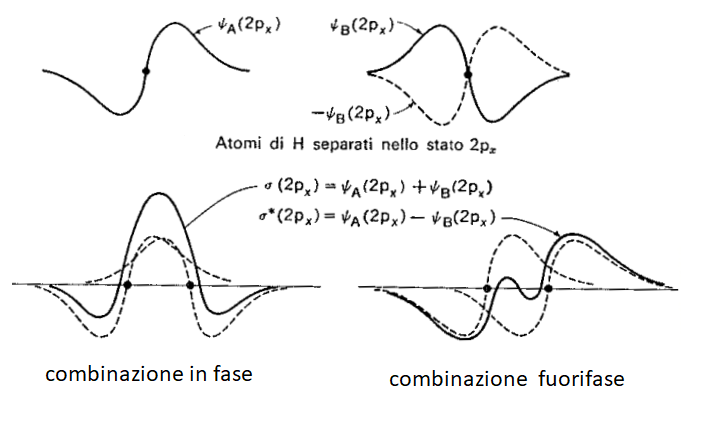
\includegraphics[width=14cm]{immagini/orbitali_molecolari_pigreco.png}
\end{figure}

\vspace{-1cm}Con "atomi di idrogeno separati nello stato 2p$_z$" si intende che gli orbitali sono stati ottenuti come soluzioni esatte dell'equazione di Schrödinger scritta per l'atomo di idrogeno, ma poi le usiamo per qualunque altro atomo. Quindi non dobbiamo scordare che quando rappresentiamo gli orbitali stiamo usando gli orbitali ottenuti per l'atomo di idrogeno, perché quelli rappresentano le soluzioni esatte. Stiamo anche pensando che sia ragionevole usare questi orbitali anche per atomi polielettronici, tenuto conto del fatto che ciò che cambia sarà la diversa penetrazione rispetto al nucleo, visto che ci saranno orbitali interni pieni e pertanto schermanti rispetto agli elettroni esterni, e dunque la diversa carica nucleare efficace sentita dagli elettroni esterni. Ne abbiamo parlato studiando la teoria atomica: noi apportiamo delle correzioni a questi sistemi, ma quando rappresentiamo le forme degli orbitali usiamo sempre gli orbitali dell'atomo di idrogeno. Quindi indipendentemente dal fatto che l'atomo di idrogeno, nel suo stato fondamentale, possiede un elettrone solo nell'orbitale 1s, per quest'atomo possiamo ottenere tutte le funzioni ($ \rm 1s, \; 2s, \; 2p, \; 3s, \; 3p, \; 3d, \; 4s, \; 4p, \; 4d, \; 4f$ e anche oltre).

\vspace{0.2cm}Se avviciniamo i due nuclei, avremo una sovrapposizione delle funzioni d'onda per quanto attiene alla combinazione lineare. Si ha un addensamento, cioè aumenta l'ampiezza della funzione d'onda lungo la congiungente i nuclei.

Se invece facciamo interagire le funzioni d'onda con segno opposto otteniamo un nodo al centro, lungo l'asse di legame, che non esiste nella combinazione in fase.

\vspace{0.2cm}Usiamo adesso la rappresentazione a nuvolette. In essa abbiamo un addensamento dei puntini della nuvoletta lungo l'asse di legame per la combinazione in fase, al contrario avremo un nodo nella combinazione fuori fase:
\newpage
\begin{figure}[htp]
    \centering
    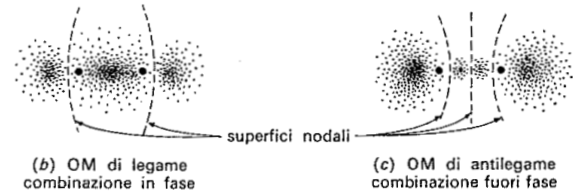
\includegraphics[width=12cm]{immagini/orbitali_molecolari_pigreco_nuvoletta.png}
\end{figure}

Va poi da ricordare che la funzione d'onda dell'orbitale p di per sé ha un nodo: essa cambia segno all'origine degli assi. Ne segue che nella combinazione in fase avremo tre lobi più i due nodi all'origine mentre nella combinazione fuori fase avremo quattro lobi e tre nodi. Graficamente:

\begin{figure}[htp]
    \centering
    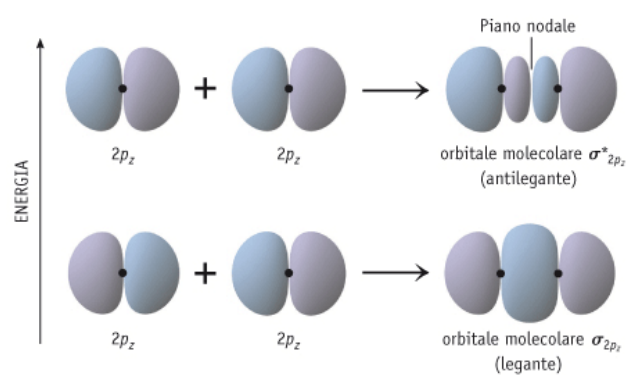
\includegraphics[width=10cm]{immagini/orbitali_sigma_p.png}
\end{figure}

Questo vale per gli orbitali che puntano lungo l'asse di legame, i quali daranno luogo a combinazioni $\sigma$ di legame e $\sigma^*$ di antilegame.

\vspace{0.2cm}Consideriamo gli orbitali p perpendicolari all'asse di legame:

\begin{figure}[htp]
    \centering
    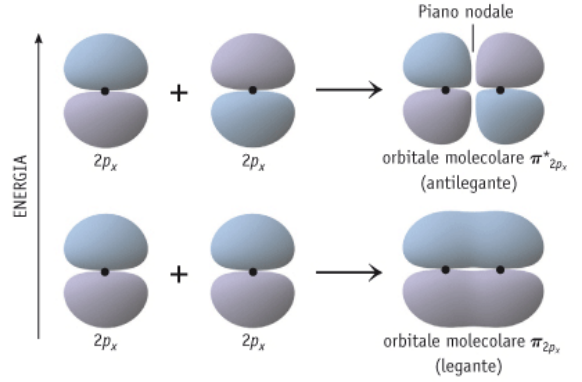
\includegraphics[width=10cm]{immagini/orbitale_pigreco_p.png}
\end{figure}
Tali orbitali daranno luogo ad una combinazione in fase, ma perpendicolarmente all'asse di legame, ossia stavolta lungo l'asse di legame ci sarà un piano nodale, e ad una combinazione fuori fase.

Gli orbitali perpendicolari all'asse di legame in totale sono quattro, quindi daranno luogo a 4 orbitali molecolari, due in fase e due fuori fase.

Non contando gli orbitali s, abbiamo tre orbitali p su ogni atomo (p$_x$, p$_y$, p$_z$) e in totale ne avremo sei, da cui segue che avremo sei orbitali molecolari: tre in fase e tre fuori fase.
In termini di energia si ha:

\begin{figure}[htp]
    \centering
    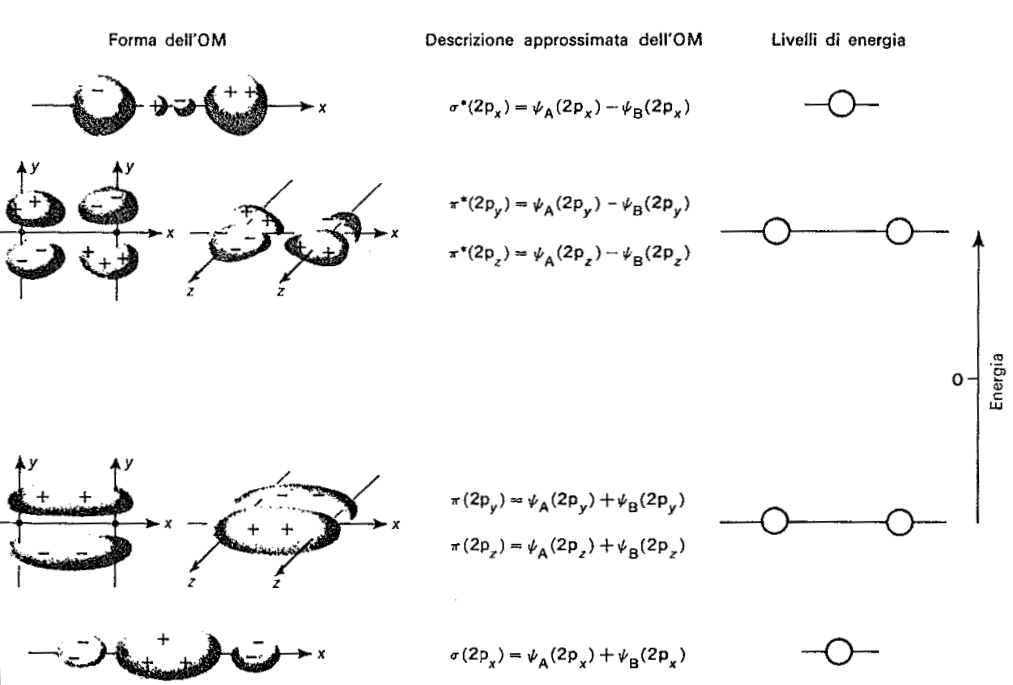
\includegraphics[width=14cm]{immagini/equazioni_orbitali.png}
\end{figure}

\vspace{0.2cm}Due orbitali p$_x$ che puntano l'uno sull'altro danno luogo alle configurazioni $\sigma_p$ di legame e $\sigma^*_p$ di antilegame, le quali da un punto di vista energetico stanno rispettivamente più in basso e più in alto.

I due set p$_y$ e p$_z$ perpendicolari all'asse di legame danno luogo alle combinazioni $\pi$ di legame e $\pi^*$ di antilegame.

Gli orbitali $\pi_{2p_y}$ e $\pi_{2p_z}$, così come avviene per i $\pi_{2p_y}^*$ e $\pi_{2p_z}^*$, sono degeneri, ossia sono allo stesso livello di energia.

In totale riempiremo gli orbitali, sia di legame che di antilegame, con 12 elettroni. Con 12 elettroni la molecola si distrugge, fino a 11 esiste.

La sequenza, dall'energia più bassa a quella più alta, degli orbitali molecolari generati a partire da orbitali p è dunque: $\sigma, \; \pi, \; \pi^*, \; \sigma^*$.
\subsection{L'anomalia di B, C, N}
Si ha però un'anomalia: boro, carbonio e azoto hanno una differenza energetica tra gli orbitali 2s e gli orbitali 2p più piccola di quella osservata subito dopo, cioè dall'ossigeno in poi.

Ragionando in kcal/mol, la differenza energetica tra gli orbitali 2s e i 2p di B, C, N è di circa 100 kcal/mol. Tale differenza arriva a 300 kcal/mol quando si arriva all'ossigeno:
\newpage
\begin{figure}[htp]
    \centering
    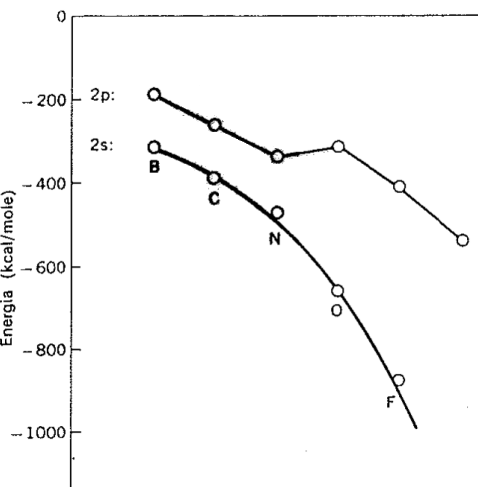
\includegraphics[width=6.5cm]{immagini/differenza_energia_2s_2p.png}
\end{figure}

Se la distanza energetica tra i livelli 2p e i livelli 2s è piccola ciò che succede è che il livello $\sigma_{2s}$ si abbassa in energia, mentre l'orbitale $\sigma_{2p}$ che è subito dopo si alza in energia a tal punto da capovolgere l'ordine, ossia quest'orbitale, interagendo con quelli più interni, si sposta fino a superare l'energia dei livelli $\pi_{2p}$. Quindi per boro, carbonio e azoto la sequenza energetica è $\pi,\; \sigma, \; \pi^*, \; \sigma^*$:

\begin{figure}[htp]
    \centering
    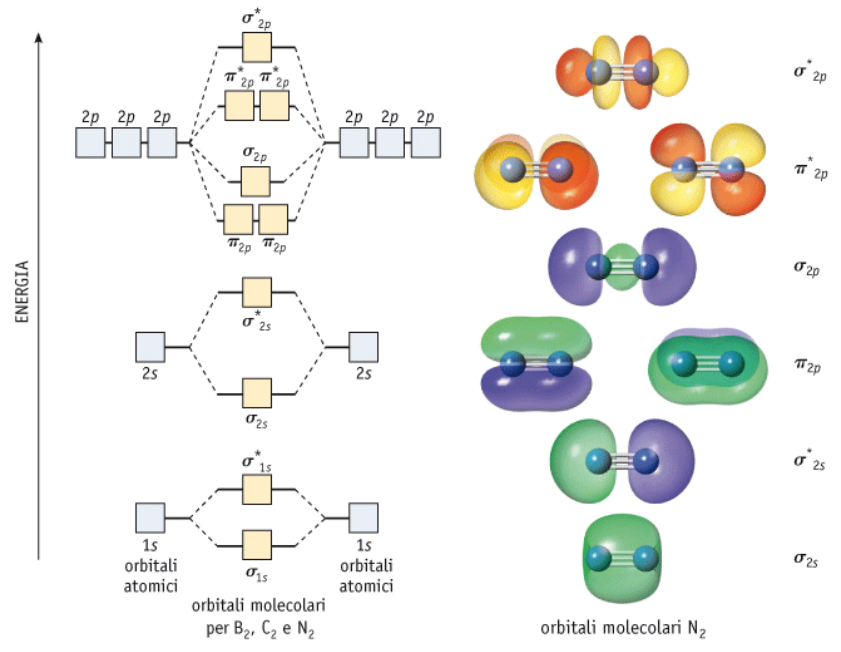
\includegraphics[width=14cm]{immagini/livelli_B2_C2_N2.png}
\end{figure}
\newpage
Vediamo in dettaglio tutte le forme degli orbitali:

\begin{figure}[htp]
    \centering
    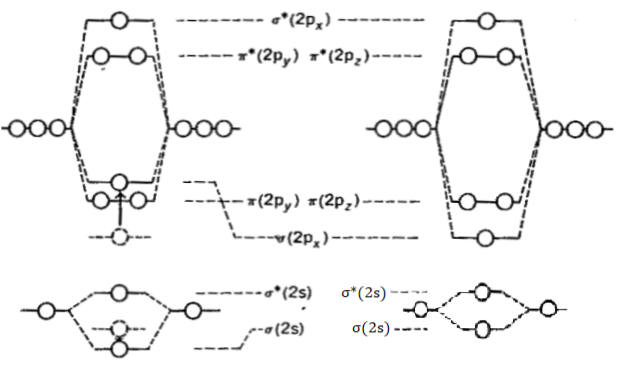
\includegraphics[width=14cm]{immagini/sequenza_energetica_BCN.png}
\end{figure}

\begin{itemize}
    \item Partendo dagli 1s, la combinazione di due di questi orbitali darà luogo ad un $\sigma$ ed un $\sigma^*$;
    \item Anche i livelli 2s danno luogo ad un $\sigma$ ed un $\sigma^*$;
    \item I tre orbitali atomici p presenti su ciascun atomo daranno luogo alle combinazioni, in ordine energetico crescente, $\pi,\; \sigma, \; \pi^*, \; \sigma^*$. A questo punto sarà solo una questione di riempimento.
\end{itemize}

Consideriamo la molecola N$_2$. Col formalismo di Lewis la rappresentavamo con un legame triplo. Contando anche i livelli 1s ogni azoto ha 7 elettroni, per un totale di 14. Se andiamo a riempire gli orbitali molecolari, arriveremo al $\sigma_{2p}$. Gli elettroni di legame sono 10, quelli di antilegame 4. L'ordine di legame è pari a (10-4)/2=3, ecco perché si usa un triplo legame per rappresentare tale molecola. Quindi con la teoria degli orbitali molecolari arriviamo alla stessa risposta ottenuta con l'approccio di Lewis.

\vspace{0.2cm}
Dall'ossigeno in poi ritorniamo al diagramma inizialmente discusso, ossia la sequenza energetica è $\sigma_{1s}, \; \sigma^*_{1s}, \; \sigma_{2s}, \; \sigma^*_{2s}, \; \sigma_{2p}, \; \pi_{2p}, \; \pi^*_{2p}, \; \sigma^*_{2p}$.

Vediamo che cosa succede alla molecola di ossigeno con questa trattazione.

Ogni ossigeno fornisce, contando anche i liveli 1s, 8 elettroni, per cui dovremo posizionare 16 elettroni. Con 14 elettroni arriviamo a riempire fino ai livelli $\pi$. I due elettroni restanti, dato che gli orbitali $\pi^*$ sono degeneri, possono stare entrambi sullo stesso orbitale oppure stanno uno su un orbitale e uno sull'altro. Queste due situazioni sono a energie diverse, in quanto se possibile gli elettroni preferiscono stare con spin paralleli in orbitali diversi. Accoppiare lo spin di due elettroni significa sempre spendere energia, quindi quando stanno nello stesso orbitale siamo a energia maggiore. Pertanto la situazione a energia più bassa si ha quando gli elettroni hanno spin paralleli ma stanno in orbitali diversi. Inoltre la situazione a più alta energia non è lo stato fondamentale dell'ossigeno.
\newpage
Ragioniamo ora in termini di molteplicità di spin, pari a $2S + 1$, dove $S$ è lo spin totale (è un numero relativo agli atomi). Questi due stati vengono chiamati stato di \textbf{tripletto} e di \textbf{singoletto}, in quanto nel caso in cui gli elettroni stiano in orbitali diversi, entrambi avranno spin pari a $\frac{1}{2}$, per cui $2 \cdot (\frac{1}{2} + \frac{1}{2})+1=2 \cdot 1 + 1=3$, mentre nel caso in cui essi siano costretti nello stesso orbitale avranno spin opposti, cioè uno spin $\frac{1}{2}$ e l'altro spin $-\frac{1}{2}$ e quindi si ha $2 \cdot (\frac{1}{2} - \frac{1}{2}) + 1= 2 \cdot 0 + 1=1$.
\begin{center}
\begin{tabular}{m{5.2cm}m{4cm}m{4cm}}
    \hspace{0.4cm}$\sigma^*_{2px}$ & \hspace{0.4cm}\vspace{-0.2cm}\orbital{0} & \hspace{0.4cm}\vspace{-0.2cm}\orbital{0}\\
    \vspace{0.4cm}$\pi^*_{2py} \quad \pi^*_{2pz}$ & \hspace{0.15cm}\vspace{-0.5cm}\orbitals{20} & \hspace{0.15cm}\vspace{-0.5cm}\orbitals{11}\\
    \vspace{0.4cm}$\pi_{2py} \quad \pi_{2pz}$ & \hspace{0.15cm}\vspace{-0.5cm}\orbitals{22} & \hspace{0.15cm}\vspace{-0.5cm}\orbitals{22}\\
    \vspace{0.4cm}\hspace{0.4cm}$\sigma_{2px}$ & \hspace{0.4cm}\vspace{-0.5cm}\orbital{2} & \hspace{0.4cm}\vspace{-0.5cm}\orbital{2}\\
    \vspace{0.4cm}\hspace{0.4cm}$\sigma^*_{2s}$ & \hspace{0.4cm}\vspace{-0.5cm}\orbital{2} & \hspace{0.4cm}\vspace{-0.5cm}\orbital{2}\\
    \vspace{0.4cm}\hspace{0.4cm}$\sigma_{2s}$ & \hspace{0.4cm}\vspace{-0.5cm}\orbital{2} & \hspace{0.4cm}\vspace{-0.5cm}\orbital{2}\\
    \vspace{0.4cm}\hspace{0.4cm}$\sigma^*_{1s}$ & \hspace{0.4cm}\vspace{-0.5cm}\orbital{2} & \hspace{0.4cm}\vspace{-0.5cm}\orbital{2}\\
    \vspace{0.4cm}\hspace{0.4cm}$\sigma_{1s}$ & \hspace{0.4cm}\vspace{-0.5cm}\orbital{2} & \hspace{0.4cm}\vspace{-0.5cm}\orbital{2}\\
    \vspace{0.4cm}Nome & \vspace{0.4cm}singoletto & \vspace{0.4cm}tripletto\\
    \vspace{0.3cm}Energia & \vspace{0.3cm}+22.5 kcal/mol & \vspace{0.3cm}0\\
    \vspace{0.3cm}Energia di legame & \vspace{0.3cm}96 kcal/mol & \vspace{0.3cm}118 kcal/mol\\
    \vspace{0.3cm}Lunghezza di legame & \vspace{0.3cm}1.22 Å & \vspace{0.3cm}1.21 Å\\
    \vspace{0.3cm}Costante di forza & \vspace{0.3cm}10.7 mdine/Å & \vspace{0.3cm}11.4 mdine/Å\\
    \vspace{0.3cm}Ordine di legame apparente & \vspace{0.3cm}2 & \vspace{0.3cm}2\\
    \vspace{0.3cm}Proprietà magnetiche & \vspace{0.3cm}non magnetico & \vspace{0.3cm}magnetico
\end{tabular}
\end{center}
Se scegliamo lo stato di tripletto come zero di energia, per ottenere lo stato di singoletto dobbiamo spendere 22.5 kcal/mol, infatti è un sistema a più alta energia cioè è meno stabile, tant'è vero che l'energia di legame è minore, la lunghezza di legame è maggiore e, immaginando il legame chimico come una molla, possiamo definire una costante di forza, che risulta minore nel singoletto. L'ordine di legame invece non cambia, perché sia quando gli elettroni stanno sullo stesso orbitale che quando stanno su orbitali diversi si trovano comunque in orbitali di antilegame. In particolare per entrambi gli stati risulta un ordine di legame pari a 2, quindi rappresentiamo l'O$_2$ con un doppio legame. 

Inoltre si ha che se gli elettroni sono appaiati (stato di singoletto) l'ossigeno sarà diamagnetico, se sono spaiati (stato di tripletto) il sistema sarà paramagnetico. Ciò è vero: l'ossigeno liquido viene trattenuto tra le espansioni di un magnete.

\vspace{0.2cm}Graficamente, la disposizione degli elettroni negli orbitali (non considerando quelli a numero quantico inferiore) è la seguente:
\begin{center}
\begin{tabular}{ m{3.2cm}m{1cm}m{1cm}m{1cm}|m{1cm}m{1cm}m{1cm}m{1cm}}
    & $\mathbf{B_2}$ & $\mathbf{C_2}$ & $\mathbf{N_2}$ & & $\mathbf{O_2}$ & $\mathbf{F_2}$ & $\mathbf{He_2}$\\
    \vspace{0.4cm}$\boldsymbol{\sigma^*}_{2p}$ & \vspace{0.2cm}\orbital{0} & \vspace{0.2cm}\orbital{0} & \vspace{0.2cm}\orbital{0} & \vspace{0.4cm}$\boldsymbol{\sigma^*}_{2p}$ & \vspace{0.2cm}\orbital{0} & \vspace{0.2cm}\orbital{0} & \vspace{0.2cm}\orbital{2}\\
    \vspace{0.4cm}$\boldsymbol{\pi^*}_{2p}$ & \hspace{-0.25cm}\vspace{-0.4cm}\orbitals{00} & \hspace{-0.25cm}\vspace{-0.4cm}\orbitals{00} & \hspace{-0.25cm}\vspace{-0.4cm}\orbitals{00} & \vspace{0.4cm}$\boldsymbol{\pi^*}_{2p}$ & \hspace{-0.25cm}\vspace{-0.4cm}\orbitals{11} & \hspace{-0.25cm}\vspace{-0.4cm}\orbitals{22} &\hspace{-0.25cm}\vspace{-0.4cm}\orbitals{22}\\
    \vspace{0.4cm}$\boldsymbol{\sigma}_{2p}$ & \vspace{0.4cm}\orbital{0} & \vspace{0.4cm}\orbital{0} & \vspace{0.4cm}\orbital{2} & \vspace{0.4cm}$\boldsymbol{\pi}_{2p}$ & \hspace{-0.25cm}\vspace{-0.4cm}\orbitals{22} & \hspace{-0.25cm}\vspace{-0.4cm}\orbitals{22} & \hspace{-0.25cm}\vspace{-0.4cm}\orbitals{22}\\
    \vspace{0.4cm}$\boldsymbol{\pi}_{2p}$ & \hspace{-0.25cm}\vspace{-0.4cm}\orbitals{11} & \hspace{-0.25cm}\vspace{-0.4cm}\orbitals{22} & \hspace{-0.25cm}\vspace{-0.4cm}\orbitals{22} & \vspace{0.4cm}$\boldsymbol{\sigma}_{2p}$ & \vspace{0.4cm}\orbital{2} & \vspace{0.4cm}\orbital{2}& \vspace{0.4cm}\orbital{2}\\
    \vspace{0.4cm}$\boldsymbol{\sigma^*}_{2s}$ & \vspace{0.4cm}\orbital{2} & \vspace{0.4cm}\orbital{2} & \vspace{0.4cm}\orbital{2} & \vspace{0.4cm}$\boldsymbol{\sigma^*}_{2s}$ & \vspace{0.4cm}\orbital{2} & \vspace{0.4cm}\orbital{2} & \vspace{0.4cm}\orbital{2}\\
    \vspace{0.4cm}$\boldsymbol{\sigma}_{2s}$ & \vspace{0.4cm}\orbital{2} & \vspace{0.4cm}\orbital{2} & \vspace{0.4cm}\orbital{2} & \vspace{0.4cm}$\boldsymbol{\sigma}_{2s}$ & \vspace{0.4cm}\orbital{2} & \vspace{0.4cm}\orbital{2} & \vspace{0.4cm}\orbital{2}\\
    \vspace{0.4cm}Ordine di legame & \vspace{0.4cm}Uno & \vspace{0.4cm}Due & \vspace{0.4cm}Tre & & \vspace{0.4cm}Due & \vspace{0.4cm}Uno & \vspace{0.4cm}Zero\\
    \vspace{0.2cm}Energia di dissociazione di legame (kJ/mol) & 290 & 620 &945 & & 498 & 155\\
    \vspace{0.2cm}Distanza di legame (pm) & 159 & 131 & 110 & & 121 & 143\\
    \vspace{0.2cm}Comportamento magnetico osservato & Para & Dia & Dia & & Para & Dia
\end{tabular}
\end{center}
I primi tre grafici sono uguali, cambia solo il riempimento degli elettroni:
\begin{itemize}
    \item Il boro è al terzo gruppo, quindi trascurando gli orbitali 1s ha 3 elettroni di valenza, per un totale di 6 nel B$_2$.
    Arriviamo a riempire parzialmente i $\pi_{2p}$, in cui gli elettroni si dispongono nei due diversi orbitali degeneri, con spinn parallelo. Ci aspettiamo allora paramagnetismo per questo sistema, cosa che effettivamente è vera. L'ordine di legame è 1, quindi la scriviamo con un legame semplice;
    \item Il carbonio avrà un elettrone in più rispetto al boro, quindi C$_2$ avrà un totale di 8 elettroni. Ne segue che stavolta riempiremo totalmente i $\pi_{2p}$. Ci aspettiamo che tale molecola sia diamagnetica, e nei fatti lo è. L'ordine di legame è $\frac{(6-2)}{2}=2$, quindi va scritta con un doppio legame;
    \item L'azoto avrà ordine di legame 3, quindi ha un triplo legame. Inoltre siccome riempiamo totalmente fino al $\sigma_{2p}$ ci aspettiamo che sia diamagnetica, cosa che nei fatti è vera;
    \item Passando dall'azoto all'ossigeno aggiungiamo ancora un elettrone, quindi in totale avremo 12 elettroni e riusciampo a riempire parzialmente fino ai livelli $\pi^*$. In particolare nella tabella è raffigurata la configurazione che fornisce paramagnetismo all'ossigeno. L'ordine di legame è 2;
    \item Nel fluoro, aggiungendo altri 2 elettroni completiamo il riempimento degli orbitali $\pi_{2p}^*$ di antilegame, per cui stiamo indebolendo il legame, tant'è che l'ordine di legame diventa $\frac{(8-6)}{2}=1$ e nei fatti l'energia di dissociazione diminuisce e la distanza di legame aumenta. Inoltre il fluoro è diamagnetico;
    \item Il neon appartiene all'ottavo gruppo, pertanto in totale avremo 16 elettroni (non contando gli $1s$), per cui riempiremo anche il livello $\sigma_{2p}^*$. Avendo riempito tutti i livelli, la molecola Ne$_2$, analogamente a He$_2$, non può esistere.
\end{itemize}
Dalla tabella notiamo che ad ordine di legame maggiore corrisponde una maggiore energia per rompere il legame e una minore distanza di legame.

\vspace{0.2cm}Consideriamo la molecola C$_2$: se è vero che il contributo al legame chimico da parte dell'orbitale $\sigma_{2s}$ viene annullato dal $\sigma_{2s}^*$ perché totalmente pieni, è anche vero che i due legami di tale molecola sono dovuti agli orbitali $\pi_{2p}$, entrambi appunto di tipo $\pi$. È quindi da sfatare la credenza che quando c'è un solo legame esso sia di tipo $\sigma$ e quando ce ne sono due il secondo sia di tipo $\pi$. Può essere così, ma non necessariamente. La molecola C$_2$ è un caso evidente in cui, essendo nullo il contributo al legame chimico dato dagli orbitali $\sigma_{2s}$, entrambi i legami sono dovuti a due diversi orbitali molecolari $\pi$ di legame.

\vspace{0.2cm}Anche nella molecola N$_2$ il contributo degli orbitali $\sigma_{2s}$ al legame chimico è nullo, ma in questo caso troveremo un legame $\sigma$ e due $\pi$ nell'ordine di legame 3.

\vspace{0.2cm}Recap: come mai dall'azoto in poi cambia la sequenza energetica?

La distanza energetica tra i livelli 2s e 2p in boro, carbonio e azoto è di appena 100 kcal/mol, mentre in ossigeno e fluoro è già di 300 kcal/mol. Nei primi tre quindi tali livelli sono energeticamente vicini, mentre negli altri due sono distanti. Laddove sono distanti non succede nulla, non si ha interazione; laddove invece i 2s sono vicini ai $2p$ succede qualcosa di diverso: finora abbiamo visto interazioni selettive (1s con 1s, 2s con 2s, 2p$_x$ con 2p$_x$, 2p$_y$ con 2p$_y$, 2p$_z$ con 2p$_z$), ma nell'istante in cui ci siano orbitali atomici che hanno la stessa simmetria pur essendo diversi, si potrà avere interazione anche tra essi, ossia non necessariamente il 2s deve interagire col 2s, può interagire anche con un 2p, purché quest'ultimo sia orientato lungo l'asse di legame. Quindi sono possibili interazioni più complesse. Nel caso specifico, nei primi tre atomi si ha una ulteriore interazione tra l'orbitale $\sigma_{2s}$ e il $\sigma_{2p}$, e questa ulteriore interazione fa si che il $\sigma_{2p}$ salga in energia fino ad andare sopra i $\pi$, mentre il $\sigma_{2s}$ scende in energia.

Si tratta quindi di una interazione addizionale che fa sì che i grafici siano diversi per B$_2$, C$_2$ e N$_2$, dove l'orbitale $\sigma_{2p}$ è più alto di quelli $\pi$, mentre per gli altri elementi è più basso, cioè il $\sigma_{2p}$ può salire o restare dov'è in funzione del fatto che i livelli $\sigma$ siano, rispettivamente, vicini o lontani.

\vspace{0.2cm}Vediamo altri esempi:
\newpage
\begin{center}
    \begin{tabular}{ m{3cm}m{1cm}m{1cm}m{1cm}m{1cm}|m{1cm}m{1cm}m{1cm}m{1cm}m{1cm}}
        & $\mathbf{C_2}$ & $\mathbf{N_2^+}$ & $\mathbf{N_2}$ & $\mathbf{N_2^-}$ & & $\mathbf{O_2^+}$ & $\mathbf{O_2}$ & $\mathbf{O_2^-}$\\
        \vspace{0.3cm}$\boldsymbol{\sigma^*}$ & \vspace{0.2cm}\orbital{0} & \vspace{0.2cm}\orbital{0} & \vspace{0.2cm}\orbital{0} & \vspace{0.2cm}\orbital{0} & \vspace{0.3cm}$\boldsymbol{\sigma^*}$ & \vspace{0.2cm}\orbital{0} & \vspace{0.2cm}\orbital{0} & \vspace{0.2cm}\orbital{0}\\
        \vspace{0.4cm}$\boldsymbol{\pi^*}$ & \hspace{-0.25cm}\vspace{-0.4cm}\orbitals{00} & \hspace{-0.25cm}\vspace{-0.4cm}\orbitals{00} & \hspace{-0.25cm}\vspace{-0.4cm}\orbitals{00} & \hspace{-0.25cm}\vspace{-0.4cm}\orbitals{10} & \vspace{0.4cm}$\boldsymbol{\pi^*}$ & \hspace{-0.25cm}\vspace{-0.4cm}\orbitals{10} & \hspace{-0.25cm}\vspace{-0.4cm}\orbitals{11} & \hspace{-0.25cm}\vspace{-0.4cm}\orbitals{21}\\
        \vspace{0.4cm}$\boldsymbol{\sigma}$ & \vspace{0.4cm}\orbital{0} & \vspace{0.4cm}\orbital{1} & \vspace{0.4cm}\orbital{2} & \vspace{0.4cm}\orbital{2}\\
        \vspace{0.4cm}$\boldsymbol{\pi}$ & \hspace{-0.25cm}\vspace{-0.4cm}\orbitals{22} & \hspace{-0.25cm}\vspace{-0.4cm}\orbitals{22} & \hspace{-0.25cm}\vspace{-0.4cm}\orbitals{22} & \hspace{-0.25cm}\vspace{-0.4cm}\orbitals{22} & \vspace{0.4cm}$\boldsymbol{\pi}$ & \hspace{-0.25cm}\vspace{-0.4cm}\orbitals{22} & \hspace{-0.25cm}\vspace{-0.4cm}\orbitals{22} & \hspace{-0.25cm}\vspace{-0.4cm}\orbitals{22}\\
        & & & & & \vspace{0.4cm}$\boldsymbol{\sigma}$ & \vspace{0.4cm}\orbital{2} & \vspace{0.4cm}\orbital{2} & \vspace{0.4cm}\orbital{2}\\
        \vspace{0.4cm}Ordine di legame & \vspace{0.4cm}2 & \vspace{0.4cm}2.5 & \vspace{0.4cm}3 & \vspace{0.4cm}2.5 & & \vspace{0.4cm}2.5 & \vspace{0.4cm}2 & \vspace{0.4cm}1.5\\
        \vspace{0.2cm}Energia di legame (kcal/mol) & \vspace{0.2cm}144 & \vspace{0.2cm}201 & \vspace{0.2cm}225 & \vspace{0.2cm}- & & \vspace{0.2cm}149 & \vspace{0.2cm}118 & \vspace{0.2cm}-\\
        \vspace{0.2cm}Lunghezza di legame (Å) & \vspace{0.2cm}1.24 & \vspace{0.2cm}1.12 & \vspace{0.2cm}1.10 & \vspace{0.2cm}- & & \vspace{0.2cm}1.12 & \vspace{0.2cm}1.21 & \vspace{0.2cm}1.28\\
        \vspace{0.2cm}Costante di forza (mdine/Å) & 9.3 & 19.5 & 22.4 & 13.2 & & 16.6 & 11.4 & 5.60
    \end{tabular}
\end{center}

\begin{itemize}
    \item Nel C$_2$ abbiamo 4 elettroni di legame, quindi l'O.L. è 2;
    \item Nel passaggio da C$_2$ a N$_2$ l'azoto ha un elettrone in più del carbonio, per cui avremo due elettroni in più. Vediamo una situazione intermedia: inizziamo l'N$_2$, generando lo ione N$_2^+$, che differisce da C$_2$ per un solo elettrone. In questo caso abbiamo 5 elettroni di legame, quindi l'O.L. è 2.5;
    \item Nell'N$_2$ abbiamo 6 elettroni di legame che danno O.L. 3;
    \item Anche tra N$_2$ e O$_2$ la differenza è di 2 elettroni. Possiamo allora avere due situazioni intermedie: nella prima togliamo un elettrone ad O$_2$, che diventa ione O$_2^+$, nella seconda cediamo un elettrone a N$_2$ che diventa ione N$_2^-$. In entrambi i casi abbiamo 6 elettroni di legame e uno di antilegame, per cui l'O.L. è 2.5;
    \item Nell'O$_2$ abbiamo 6 elettroni di legame e due di antilegame, quindi l'O.L. sarà 2;
    \item Possiamo poi cedere un elettrone a O$_2$, ottenendo lo ione O$_2^-$. In esso abbiamo 6 elettroni di legame e 3 di antilegame, quindi l'O.L. sarà 1.5.
\end{itemize}

In tutte queste molecole al diminuire dell'O.L. diminuiscono l'energia di legame e la costante di forza, mentre aumenta la distanza di legame.

Tutti i dati sono in accordo con le previsioni del modello che stiamo utilizzando, cioè tramite la teoria degli orbitali molecolari siamo in grado di ottenere dei dati che non sono soluzioni esatte di una equazione che non sappiamo risolvere, ma che sono soluzioni estremamente vicine a quelle che ci aspetteremmo qualora fossimo in grado di ottenerle da un punto di vista teorico con metodi di calcolo estremamente accurati, cioè le approssimazioni raggiunte oggi sono prossime a delle soluzioni non esatte ma quantomeno precise dei modelli quanto-meccanici di calcolo.

\subsection{Molecole eteronucleari}
Finora abbiamo fatto interagire selettivamente orbitali dello stesso tipo. Abbiamo fatto ciò perché avevamo atomi identici e quindi ogni livello ne aveva un altro accanto alla stessa energia.

Supponiamo di avere due atomi molto diversi. Vale ancora questo discorso, cioè l'1s$_A$ interagirà con l'1s$_B$ e così via?

Entriamo quindi nel merito delle quattro informazioni necessarie per costruire gli orbitali molecolari anche per sistemi per i quali le posizioni energetiche degli orbitali atomici dello stesso tipo sono molto diverse. È il caso tipico di molecole ottenute da atomi con elettronegatività parecchio diversa.

\vspace{0.2cm}$\bullet$\textbf{ES.1} HF

Consideriamo la molecola dell'acido fluoridrico, che abbiamo etichettato come covalente polare. Cosa succederà? L'unico orbitale occupato nello stato fondamentale dell'idrogeno, ossia l'1s, interagirà con l'1s del fluoro?

\vspace{0.2cm}Servono delle affermazioni che ci saranno da guida per costruire diagrammi di orbitali molecolari:

\begin{enumerate}
    \item Gli orbitali atomici interagiranno in fase e fuori fase e genereranno orbitali molecolari;
    \item Il numero di orbitali molecolari ottenuti sarà sempre uguale al numero di orbitali atomici interagenti;
    \item L'orbitale molecolare si estenderà sull'intera molecola. Ne segue che il legame localizzato perde significato: l'elettrone sarà localizzato sull'intera molecola;
    \item Gli orbitali che interagiranno saranno quelli che hanno la stessa simmetria ma anche energia confrontabile: se hanno la stessa simmetria ma stanno ad energie lontane non si avrà interazione.
\end{enumerate}

\begin{figure}[htp]
    \centering
    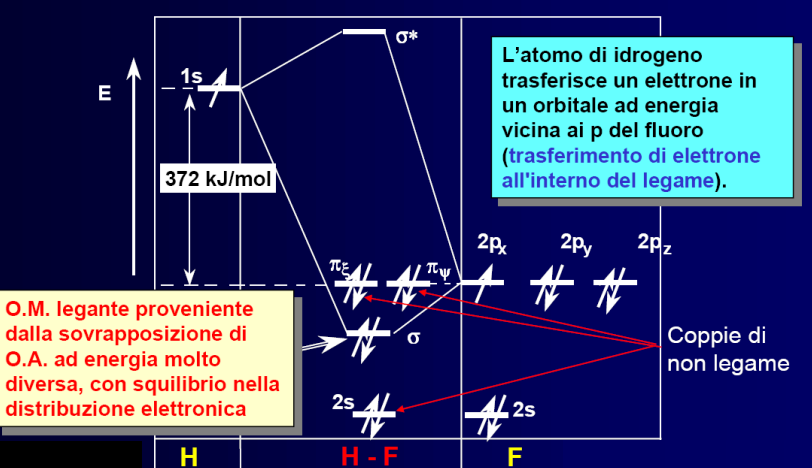
\includegraphics[width=10cm]{immagini/orbitali_molecolari_HF.png}
\end{figure}

Consideriamo le energie dei livelli atomici. Si nota che l'1s del fluoro non è nemmeno riportato, perché è molto interno in energia (e non è nemmeno di valenza), mentre l'1s dell'idrogeno si.

Anche l'orbitale 2s del fluoro è molto distante, quindi pur avendo la stessa simmetria (sono entrambi orbitali di tipo s) non ci sarà interazione con l'1s dell'idrogeno perché molto distanti in energia.

Gli orbitali del fluoro più vicini in energia all'1s dell'idrogeno sono orbitali di tipo p, quindi l'interazione si avrà tra l'orbitale 1s dell'idrogeno e quell'orbitale p del fluoro che giace lungo l'asse di legame H-F. Se allora scegliamo l'asse $x$ come asse di legame, l'orbitale 2p$_x$ sarà quello i cui lobi puntano lungo l'asse di legame e sarà quest'orbitale a interagire con l'1s dell'idrogeno. Gli altri due orbitali 2p$_y$ e 2p$_z$ sono perpendicolari a quest'asse, e siccome non hanno partners in simmetria (sull'idrogeno non abbiamo orbitali perpendicolari all'asse di legame) non verranno coinvolti nel legame chimico, pertanto li troveremo alla stessa energia, solo che adesso saranno orbitali $\pi$ nonostante le funzioni d'onda non si siano mescolate, infatti è improprio parlare di livelli $\pi$ perché non sono funzioni d'onda molecolari, bensì atomiche perché non si sono mescolate con alcun orbitale dell'atomo di idrogeno, in quanto non ce ne sono di adatti.

Quindi avremo interazione solo tra il livello 2p$_x$ del fluoro e l'1s dell'idrogeno, i quali daranno luogo alla combinazione in fase e quella fuori fase, che sono orbitali di tipo $\sigma$ e $\sigma^*$ perché ottenuti da un orbitale s e uno p che giace sull'asse di legame.

\vspace{0.2cm}Queste considerazioni sono state fatte a priori del riempimento.

Supponiamo ora che sull'orbitale 2p$_x$ ci sia un elettrone. Esso, insieme a quello che sta sull'1s, andrà a occupare l'orbitale più basso in energia che è il $\sigma$. C'è quindi un guadagno a formare questa molecola perché i due elettroni si stabilizzano in energia. Resta invece vuoto il $\sigma^*$.

Le due coppie di elettroni a più alta energia negli orbitali 2p$_y$ e 2p$_z$ non sono in orbitali molecolari, sono in orbitali atomici che non hanno interagito con alcun orbitale dell'atomo di idrogeno. Anche il 2s del fluoro è alla stessa energia di partenza perché, pur essendo adatto vista la sua simmetria ad interagire con un altro orbitale s, è ad energia estremamente più bassa, quindi non c'è possibilità che interagiscano perché molto lontani in energia.

Questo era un primo esempio di interazione tra orbitali di atomi diversi a energia diversa. Inoltre come si evince dal diagramma questa interazione non è molto grande: rispetto all'energia dei livelli 2p, il livello $\sigma$ si stabilizza (cioè scende in energia) di poco e rispetto all'1s il $\sigma^*$ si destabilizza (cioè sale in energia) di poco ma in egual quantità, così da mantenere il baricentro in energia. Ciò avviene perché le energie in gioco sono molto diverse. Se le energie degli orbitali interagenti fossero più vicine ci sarebbe più interazione, e i livelli $\sigma$ e $\sigma^*$ si stabilizzerebbero e destabilizzerebbero di più. In questo caso quindi l'interazione è contenuta, per cui nel riempire possiamo dire che gli elettroni 2s del fluoro resteranno tali, cioè non si mescolano, e analogamente per i livelli 2p$_y$ e 2p$_z$. L'unico mescolamente si ha tra i livelli 2p$_x$ e 1s, che danno luogo ai livelli $\sigma$ e $\sigma^*$. Va però da aggiungere che il livello $\sigma$ di legame ricorderà molto nel suo carattere l'orbitale di partenza. Ciò significa che se l'orbitale molecolare è vicino al p$_x$ del fluoro, quando contiene 2 elettroni (quindi anche quello che prima era dell'idrogeno) implicitamente diciamo che l'elettrone dell'idrogeno non viene trasferito, ma certamente spostato sul fluoro. Quindi mentre prima questo concetto veniva fuori dall'elettronegatività, ora viene fuori dalla teoria degli orbitali molecolari, cioè: avevamo due elettroni (trascurati quelli che non prendono parte alle interazioni del legame chimico), uno sull'idrogeno e uno sul fluoro, ora sono entrambi su un orbitale che però energeticamente è vicino a quello di partenza del fluoro, mentre il livello vicino al livello di partenza dell'idrogeno si è svuotato. Quindi la composizione dell'autovettore del livello $\sigma$ ha all'80-90\% il carattere del 2p$_x$ del fluoro e solo per il 10\% quello dell1s dell'idrogeno. Al contrario per il $\sigma^*$: avrà l'80-90\% del carattere dell' 1s dell'idrogeno e solo il 10\% del 2p$_x$ del fluoro. Ciò significa che il mescolamento è stato scarso, ma un elettrone alla fine è stato quasi spostato dall'idrogeno al fluoro. Non diciamo trasferito per il fatto che, anche se in minima parte, persiste il carattere dell'1s, quindi l'elettrone non è ceduto ma spostato in larga misura su livelli basati sul fluoro (questa cosa veniva rappresentata con una nuvoletta più densa sul fluoro e meno densa sull'idrogeno).

\vspace{0.2cm}Vediamo infine un recap su quali siano i casi in cui si formano i legami:
\begin{itemize}
    \item Due orbitali s, centrosimmetrici e sferici, interagiranno dando sempre luogo a orbitali $\sigma$; 
    \item Due orbitali p che puntano l'uno sull'altro danno luogo a orbitali $\sigma$;
    \item Anche un orbitale s e uno p possono dare luogo ad una interazione $\sigma$;
    \item Anche gli orbitali d, purché abbiano lobi che puntano l'uno sull'altro e dello stesso segno, danno luogo a orbitali $\sigma$ di legame;
    \item Due orbitali p che hanno un nodo lungo l'asse di legame danno luogo ad un legame $\pi$;
    \item Due orbitali d che hanno stesso segno ma un nodo lungo l'asse di legame danno luogo ad un legame $\pi$.
\end{itemize}

Abbiamo visto che il diagramma qualitativo ottenuto per alcune molecole biatomiche omonucleari, distinguendole tra B$_2$, C$_2$, N$_2$ e O$_2$, F$_2$, Ne$_2$, in funzione del livello di energia dell'orbitale $\sigma$ proveniente dalla combinazione lineare degli orbitali p, ci dava delle previsioni che concordano coi valori sperimentali di energia di legame, lunghezza di legame e costante di forza del legame. Usando poi il concetto di ordine di legame vedevamo che nelle molecole B$_2$, C$_2$, N$_2$  l'O.L. cresce di una unità alla volta. Inoltre in esse aumentano energia e costante di forza, mentre diminuisce la lunghezza di legame. Dopodiché per O$_2$, F$_2$ e Ne$_2$ avviene il contrario: O.L., energia e costante di forza diminuiscono, mentre la distanza di legame cresce.

Le osservazioni fatte si ripetono scendendo lungo i gruppi a cui appartengono le varie molecole, cioè hanno validità generale, in quanto si tratta di razionalizzazioni di esiti di calcoli quanto-meccanici abbastanza accurati.

Fin qui le molecole studiate sono omonucleari, cioè fatte da atomi identici, cosa che comporta l'avere gli stessi livelli energetici interagenti, cioè i vari livelli 1s, 2s, 2p ecc. sono alla stessa energia. Se invece consideriamo sistemi ancora biatomici ma eteronucleari, cambierà la posizione relativa dei livelli energetici degli atomi, il che significa che all'aumentare del numero atomico si abbassa l'energia dei livelli elettronici (infatti nel caso dell'HF il livello 1s dell'idrogeno è paragonabile in energia ai livelli 2p del fluoro).

Un caso limite in cui il legame è covalente ma fortemente polare (cioè in cui c'è una grande differenza di elettronegatività) è la molecola HF. Con l'approccio quanto-meccanico abbiamo visto che l'orbitale 1s del fluoro, che non è di valenza, è ad energia estremamente più bassa rispetto a quella dell'orbitale 1s dell'idrogeno. Siccome ai fini del legame chimico dobbiamo considerare principlamente gli orbitali di valenza dei vari atomi, per quanto attiene al fluoro considereremo l'orbitale 2s e i tre 2p, trascurando l'1s.

Visto che il numero atomico del fluoro è maggiore di quello dell'idrogeno, tutti gli orbitali di valenza del fluoro saranno ad energia più bassa dell'orbitale di valenza dell'idrogeno. Se non conoscessimo la posizione energetica di questi livelli, inizialmente potremmo pensare che l'interazione principale avvenga tra il livello 1s dell'idrogeno e il 2s del fluoro dato che hanno la stessa simmetria. Nei fatti questa interazione c'è, ma è scarsa e quindi non viene riportata. È scarsa a causa della elevata differenza di energia tra questi livelli, ossia l'orbitale 2s del fluoro è molto interno in energia, quindi ad energia parecchio negativa. Risultano invece essere più vicini all'energia del livello 1s dell'idrogeno gli orbitali 2p del fluoro. Quindi le interazioni di legame, se possibili, avverranno tra i 2p del fluoro e l'1s dell'idrogeno. Inoltre dei tre livelli p solo uno punta lungo l'asse di legame, gli altri due sono perpendicolari all'asse. Non essendoci orbitali perpendicolari all'asse sull'atomo di idrogeno, gli orbitali 2p rimarranno non coinvolti nel legame chimico, restano orbitali atomici. L'orbitale diretto lungo l'asse di legame invece darà luogo alle combinazioni in fase e fuori fase di orbitali molecolari. Dunque i tre orbitali p del fluoro nei fatti si separano in un set dovuto all'orbitale parallelo all'asse, l'altro dovuto agli orbitali perpendicolari all'asse, i quali resteranno atomici (e alla stessa energia). Pertanto l'unica interazione realmente presente in questo sistema è quella tra l'orbitale 2p del fluoro parallelo all'asse e l'orbitale 1s dell'atomo di idrogeno, che è di tipo $\sigma$. Inoltre a causa della significativa differenza di energia tra questi due livelli, l'interazione pur se possibile non è forte, per cui le combinazioni in fase e fuori dase daranno luogo ad orbitali molecolari che fortemente ricordano per energia e per carattere gli orbitali atomici di partenza. Nel caso particolare dell'HF l'orbitale molecolare $\sigma$ avrà un forte carattere del fluoro, cioè la composizione dell'autovettore è fortemente localizzata sul fluoro pur avendo una certa percentuale di carattere dell'1s dell'idrogeno, cioè il mescolamento c'è stato ma scarso. Analogamente, il $\sigma^*$ avrà un forte carattere dell'orbitale 1s dell'idrogeno.

Da questa descrizione viene fuori che, avendo i due orbitali interagenti un elettrone ciascuno ed andando entrambi gli elettroni ad occupare il livello più basso in energia ossia l'orbitale $\sigma$ di legame, nei fatti ciò comporta un forte trasferimento di quest'elettrone dapprima appartenente solo all'atomo di idrogeno, su un orbitale fortemente localizzato sul fluoro. Pertanto ciò che chiamavamo "spostamento di carica di legame dovuto all'elettronegatività" adesso risulta essere un trasferimento dovuto al fatto che entrambi gli elettroni appartenenti a questo orbitale sono fortemente localizzati sul fluoro, cioè l'autovettore della funzione $\sigma$ ricorda molto il 2p del fluoro. In questo modo vediamo che c'è un forte trasferimento dell'elettrone dell'idrogeno ad un orbitale fortemente localizzat sul fluoro.

Quindi tutte le volte che avremo a che fare con molecole eteronucleari dovremo ricordare che non c'è più esatta condivisione degli elettroni di legame, la quale non si basa più sul concetto di elettronegatività ma su evidenze quanto-meccaniche.

\vspace{0.4cm}Consideriamo adesso varie molecole eteronucleari:
\newpage
\begin{center}
    \begin{tabular}{m{3.4cm}m{1cm}m{1cm}m{1cm}m{1cm}|m{1cm}m{1cm}m{1cm}m{1cm}m{1cm}}
        & $\mathbf{C_2}$ & \hspace{-0.1cm}$\mathbf{CN}$ & $\mathbf{N_2}$ & \hspace{-0.5mm}$\mathbf{CO}$ & & \hspace{-0.5mm}$\mathbf{NO}$ & $\mathbf{O_2}$\\
        \vspace{0.4cm}$\boldsymbol{\sigma^*}$ & \vspace{0.2cm}\orbital{0} & \vspace{0.2cm}\orbital{0} & \vspace{0.2cm}\orbital{0} & \vspace{0.2cm}\orbital{0} & \vspace{0.4cm}$\boldsymbol{\sigma^*}$ & \vspace{0.2cm}\orbital{0} & \vspace{0.2cm}\orbital{0}\\
        \vspace{0.4cm}$\boldsymbol{\pi^*}$ & \hspace{-0.25cm}\vspace{-0.4cm}\orbitals{00} & \hspace{-0.25cm}\vspace{-0.4cm}\orbitals{00} & \hspace{-0.25cm}\vspace{-0.4cm}\orbitals{00} & \hspace{-0.25cm}\vspace{-0.4cm}\orbitals{00} & \vspace{0.4cm}$\boldsymbol{\pi^*}$ & \hspace{-0.25cm}\vspace{-0.4cm}\orbitals{10} & \hspace{-0.25cm}\vspace{-0.4cm}\orbitals{11}\\
        \vspace{0.4cm}$\boldsymbol{\sigma}$ & \vspace{0.4cm}\orbital{0}  & \vspace{0.4cm}\orbital{1} & \vspace{0.4cm}\orbital{2} & \vspace{0.4cm}\orbital{2}\\
        \vspace{0.4cm}$\boldsymbol{\pi}$ & \hspace{-0.25cm}\vspace{-0.4cm}\orbitals{22} & \hspace{-0.25cm}\vspace{-0.4cm}\orbitals{22} & \hspace{-0.25cm}\vspace{-0.4cm}\orbitals{22} & \hspace{-0.25cm}\vspace{-0.4cm}\orbitals{22} & \vspace{0.4cm}$\boldsymbol{\pi}$ & \hspace{-0.25cm}\vspace{-0.4cm}\orbitals{22} & \hspace{-0.25cm}\vspace{-0.4cm}\orbitals{22}\\
        & & & & & \vspace{0.4cm}$\boldsymbol{\sigma}$ & \vspace{0.4cm}\orbital{2} & \vspace{0.4cm}\orbital{2}\\
        \vspace{0.4cm}Ordine di legame & \vspace{0.4cm}2 & \vspace{0.4cm}2.5 & \vspace{0.4cm}3 & \vspace{0.4cm}3 & & \vspace{0.4cm}2.5 & \vspace{0.4cm}2\\
        \vspace{0.2cm}Energia di legame (kcal/mol) & \vspace{0.2cm}144 & \vspace{0.2cm}188 & \vspace{0.2cm}225 & \vspace{0.2cm}256 & & \vspace{0.2cm}151 & \vspace{0.2cm}118\\
        \vspace{0.2cm}Lunghezza di legame (Å) & \vspace{0.2cm}1.24 & \vspace{0.2cm}1.18 & \vspace{0.2cm}1.10 & \vspace{0.2cm}1.13 & & \vspace{0.2cm}1.15 & \vspace{0.2cm}1.21\\
        \vspace{0.2cm}Costante di forza (mdine/Å) & \vspace{0.2cm}9.3 & \vspace{0.2cm}15.8 & \vspace{0.2cm}22.4 & \vspace{0.2cm}18.6 & & \vspace{0.2cm}15.5 & \vspace{0.2cm}11.4
    \end{tabular}
\end{center}

Concentriamoci sul monossido di carbonio:

\vspace{0.2cm}$\bullet$\textbf{ES.2}: CO

\begin{figure}[htp]
    \centering
    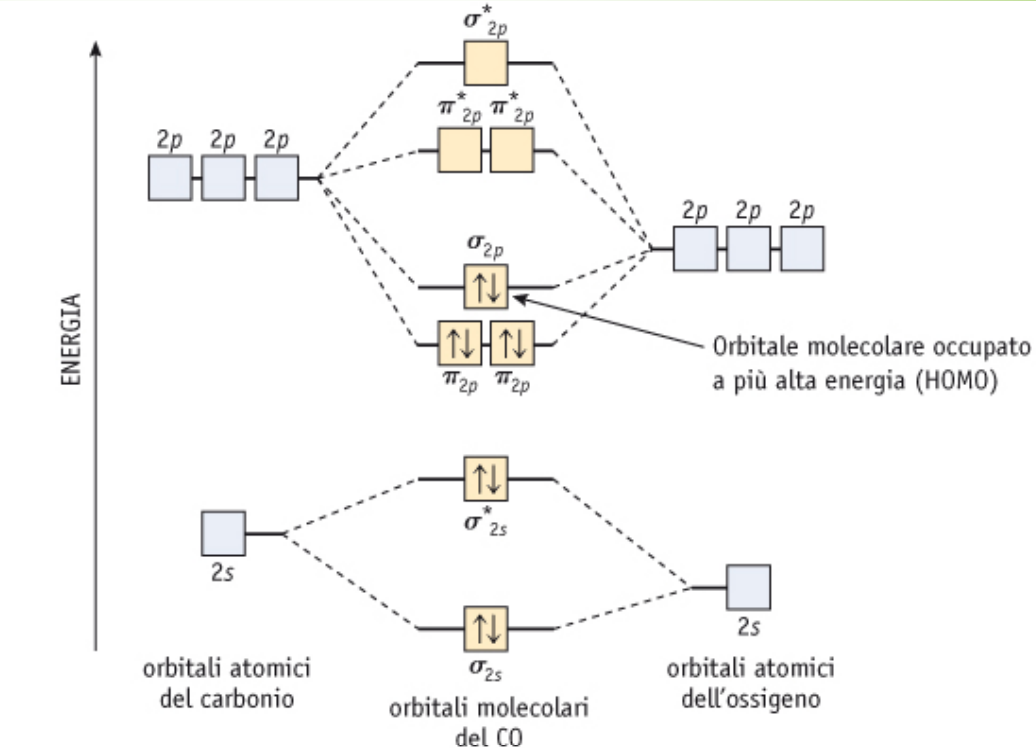
\includegraphics[width=10cm]{immagini/orbitali_molecolari_CO.png}
\end{figure}

A sinistra abbiamo gli orbitali del carbonio, a destra quelli dell'ossigeno. I livelli 1s non vengono rappresentati perché non di valenza.

Questo grafico qualitativo dell'energia ci mostra che il livello $\rm 2s$ dell'ossigeno è più basso rispetto al 2s del carbonio. Altrettanto vale per le energie dei livelli 2p, cioè l'energia del 2p dell'ossigeno è più bassa rispetto a quella del 2p del carbonio. Questo perché l'ossigeno ha un numero atomico maggiore, e avendo un nucleo con più protoni gli elettroni degli stessi livelli risultano più attratti, più legati e quindi più vicini al nucleo, pertanto ad energia più bassa.

Nel diagramma di energia avremo il livello $\sigma_{2p}$ più alto in energia dei livelli $\pi_{2p}$, perché la molecola considerata ha un atomo di carbonio, nel quale vi è una differenza di energia piccola tra i livelli 2s e 2p (circa 100 kcal/mol).

Abbiamo 4 elettroni di valenza sul carbonio e 6 sull'ossigeno, per un totale di 10 elettroni. Dunque riempiremo tutti i livelli completamente fino al $\sigma_{2p}$. Gli elettroni di legame sono 6, quelli di antilegame sono 2, per cui l'O.L. è 3, come quello della molecola N$_2$. Infatti si dice che CO e N$_2$ sono molecole isoelettroniche.

Se guardiamo la sequenza, anche per le molecole eteronucleari all'aumentare dell'O.L. corrisponde un aumento dell'energia di legame e della costante di forza, mentre la lunghezza di legame diminuisce.

\vspace{0.2cm}Consideriamo ora una molecola con 3 atomi, l'ozono O$_3$.

\vspace{0.2cm}$\bullet$\textbf{ES.3}: O$_3$

\begin{figure}[H]
    \centering
    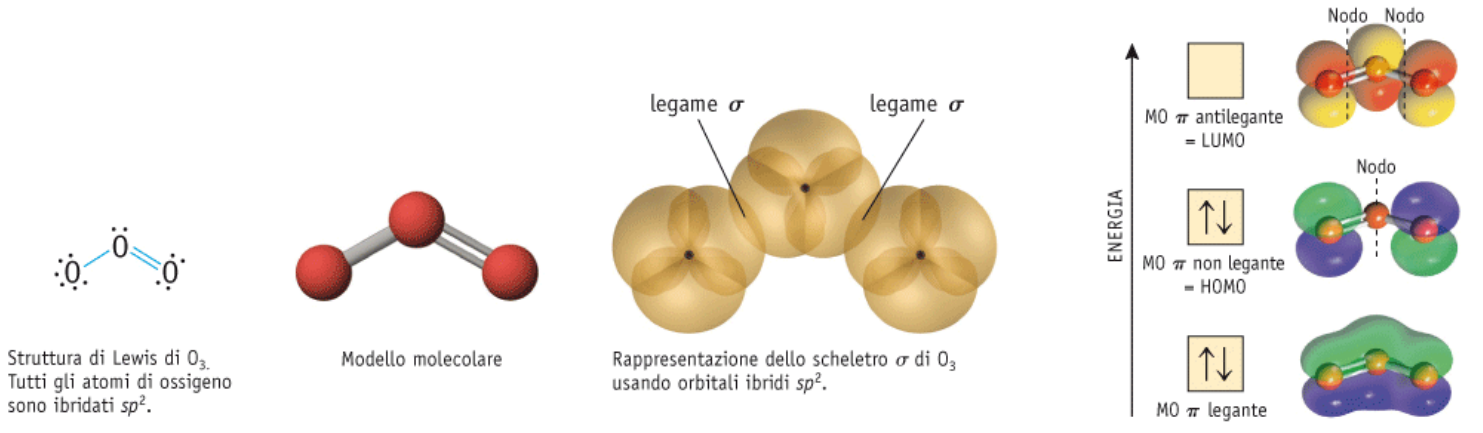
\includegraphics[width=14cm]{immagini/orbitali_molecolari_O_3.png}
\end{figure}

L'ossigeno è al sesto gruppo, per cui ha 6 elettroni di valenza e dunque in totale avremo 18 elettroni.

Il formalismo di Lewis ci diceva di mettere un atomo al centro, due ai lati ed iniziare a legarli. In questo modo consumavamo 4 elettroni e ne restavano 14. A questo punto davamo 6 elettroni all'atommo sinistro, 6 a quello destro e 2 a quello centrale. Poiché quest'ultimo in questo modo non raggiungeva l'ottetto, prendevamo un doppietto qualunque di uno dei due atomi periferici e lo trasformavamo in doppio legame, così che anche l'atomo centrale raggiungesse l'ottetto.

Ragioniamo in termini di orbitali molecolari.

Tre punti individuano un piano, pertanto O$_3$ è una molecola planare. Se immaginiamo che gli orbitali 2s e 2p dell'ossigeno siano ibridizzati, dato che la molecola è planare l'ibridizzazione è di tipo sp$^2$. Ciò significa che un orbitale s e due dei tre orbitali p di ogni atomo si mescolano per dar luogo a tre orbitali ibridi per ciascun atomo:

\begin{figure}[htp]
    \centering
    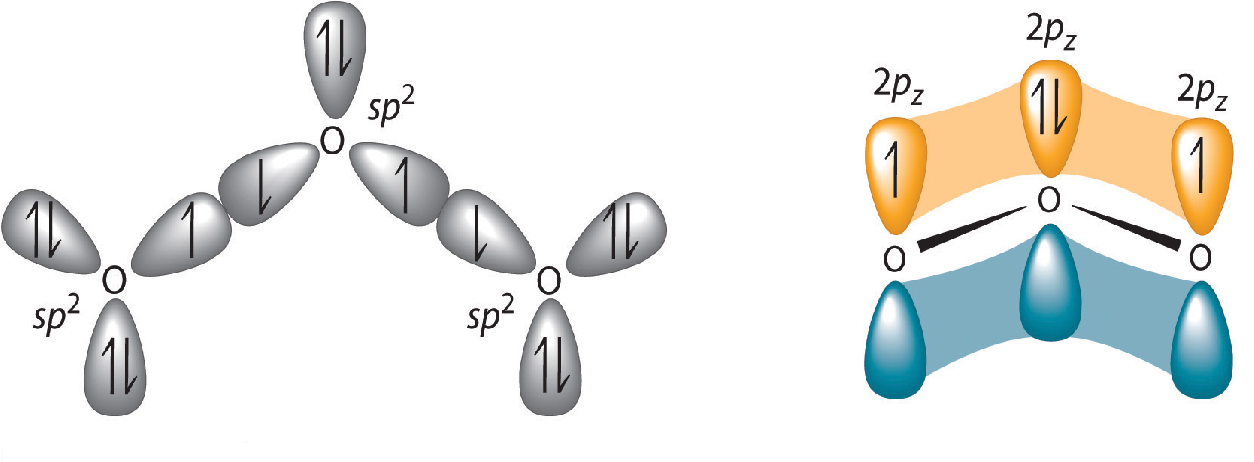
\includegraphics[width=9cm]{immagini/orbitali_ibridi_O_3.png}
\end{figure}

4 orbitali di questi tre atomi formano i due legami $\sigma$, gli altri orbitali invece conterranno le coppie solitarie. Con questo sistema allochiamo 14 elettroni, ne restano 4. La teoria dell'ibridizzazione dice che, se un atomo mescola il suo orbitale 2s con due dei suoi orbitali p per ottenere ibridi sp$^2$, il terzo orbitale resterà non ibridizzato, quindi atomico, ma perpendicolare alla molecola, per cui ogni atomo di ossigeno avrà ancora un orbitale p perpendicolare al piano della molecola, dunque avremo 3 orbitali in cui sistemare i 4 elettroni.

Quando il numero di orbitali che interagiscono tra di loro è dispari, si ottiene la combinazione in fase e quella fuori fase, mentre un orbitale non partecipa. Esso prende il nome di \textbf{non legante}. Essi si ottengono dai 3 orbitali perpendicolari al piano, per cui daranno luogo ad orbitali molecolari $\pi$ (interagiscono sopra e sotto il piano molecolare). In definitiva quindi avremo un orbitale $\pi$ di legame, uno $\pi$ di non legame e uno $\pi$ di antilegame dovuti agli orbitali p non coinvolti nella ibridizzazione sp$^2$.

Dei 4 elettroni rimanenti, 2 vanno a occupare l'orbitale di legame, quindi si formerà un secondo legame (a carattere $\pi$) localizzato arbitrariamente. Infatti dicevamo che questo secondo legame si ripartisce su tutta la molecola e l'O.L. era pari a 1.5 per entrambi i legami, anziché 1 per un legame e 2 per l'altro, fatto in accordo coi dati sperimentali in quanto si osservano gli stessi valori in entrambi i legami. Quindi anche con gli orbitali molecolari otteniamo gli stessi risultati che si trovavano con l'approccio di Lewis.

Inoltre, avendo un doppietto sull'atomo centrale non possiamo aspettarci una molecola lineare (altrimenti sarebbe stato un sistema tipo CO$_2$). Infatti la coppia solitaria respinge le coppie legate, per cui la molecola O$_3$ non può essere lineare: deve essere piegata ed avrà O.L. pari a 1.5 perché questi elettroni di non legame non contribuiscono al legame, né a favore, né a sfavore, perciò non si contano.

Se andiamo a vedere le forme degli orbitali, nella combinazione in fase i lobi degli orbitali p perpendicolari al piano della molecola, centrati su ciascuno degli atomi dell'ossigeno, hanno lo stesso segno sia sopra che sotto (ad es. tutti positivi sopra e tutti negativi sotto); nella combinazione fuori fase invece i lobi hanno segni opposti alternati; infine nella combinazione di non legame uno dei tre orbitali non partecipa e gli altri due hanno lobi di segno opposto.

\vspace{0.2cm}$\bullet$\textbf{ES.4} Benzene C$_6$H$_6$

Il benzene è usato nelle benzine per il suo elevato potere antidetonante in sostituzione al piombo tetraetile. Fa parte dei composti aromatici, i quali sono così detti perché hanno caratteristiche e un particolare assetto di elettroni che seguono le seguenti regole:

\begin{itemize}
    \item la sua struttura è ciclica, cioè chiusa in sé stessa;
    \item Tutti gli atomi del ciclo sono ibridizzati sp$^2$, per cui la struttura sarà planare con gli orbitali p non ibridizzati ortogonali al piano della molecola;
    \item Il numero di elettroni negli orbitali p deve essere pari a 4n+2 con n $\in \mathbb{N}$ (regola di Huckel)
\end{itemize}

Per via del fatto che è una molecola planare con formula C$_6$H$_6$, spesso il benzene viene descritto come un esagono all'interno del quale ci saranno tre doppi legami. Ogni vertice dell'esagono sta ad indicare una coppia C-H, o meglio il carbonio occupa il vertice e ad ogni carbonio è legato anche un atomo di idrogeno.

Essendo planare, il carbonio avrà ibridizzazione $\rm sp^2$, cioè l'orbitale s e due orbitali p (quelli che individuano il piano su cui giace la molecola) si mescolano per dar luogo a tre orbitali ibridi. In totale dunque avremo 18 orbitali ibridi. Ogni atomo di carbonio userà un orbitale ibrido per legare un idrogeno e due orbitali ibridi per legare gli atomi di carbonio ad esso adiacenti. In questo modo ogni atomo di carbonio usa tutti e tre gli orbitali $\rm sp^2$, che formano lo scheletro $\sigma$.

In questo modo si ottengono 6 legami C-C e 6 legami C-H. Resta su ogni atomo di carbonio un orbitale p non ibridizzato perpendicolare al piano individuato dai sei atomi, cioè al piano molecolare, su cui è presente un elettrone, perché a seguito dello stato di promozione del carbonio i suoi 4 elettroni esterni si disporranno uno su ogni orbitale: uno sul 2s e uno su ciascuno dei tre 2p, quindi ce ne sarà uno anche sull'orbitale non ibridizzato. Pertanto avremo sei orbitali non ibridizzati di tipo p perpendicolari al piano molecolare, i quali daranno luogo a sei orbitali molecolari: tre combinazioni saranno di legame, tre di antilegame. Tutti e sei però avranno carattere $\pi$ perché essendo perpendicolari al piano, l'interazione avviene sopra e sotto questo, mentre su di esso conterranno nodi.

Consideriamo il diagramma in energia:

\begin{figure}[htp]
    \centering
    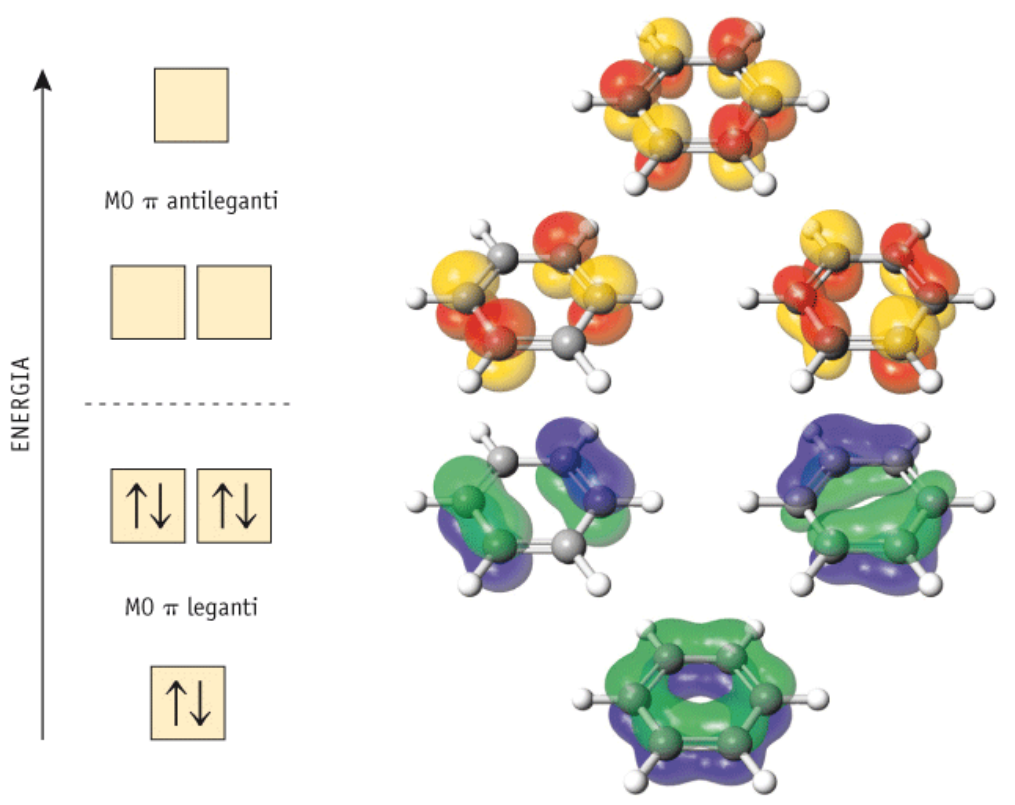
\includegraphics[width=8cm]{immagini/orbitali_molecolari_benzene.png}
\end{figure}

Come riferimento, cioè come zero in energia si prende l'energia degli orbitali atomici non ancora interagenti.

Avremo le combinazioni in fase ad energia più bassa e quelle fuori fase ad energia più alta.
        
Abbiamo però solo 6 elettroni da sistemare, per cui riempiamo soltanto 3 orbitali leganti di cui uno è a energia più bassa e gli altri due a energia un po' più alta. 
    
Quindi questi 6 orbitali p perpendicolari al piano molecolare danno luogo a 6 orbitali molecolari $\pi$ fra i quali solo i 3 di legame sono riempiti. Pertanto oltre allo scheletro $\sigma$ che ci dà i legame semplici C-C e C-H abbiamo altri tre legami da sistemare all'interno dell'esagono, i quali costituiranno gli orbitali $\pi$.
    
Spesso si rappresentano questi legami alternando legami singoli e legami doppi, cioè vengono disposti in modo alternato all'interno dell'esagono. La scelta su quali legami siano singoli e quali doppi è arbitraria, per cui spesso la molecola viene rappresentata con un anello all'interno per dire che gli orbitali molecolari si estendono sull'intera molecola, la quale gode dunque di tre parziali doppi legami, cioè non abbiamo legami doppi e legami semplici: ogni legame avrà ordine 1.5. Questo è ciò che sperimentalmente si osserva, cioè tutti i legami sono identici.

Nella combinazione in fase abbiamo una funzione d'onda $\Psi$ che è combinazione di  $\phi_1 , \; \phi_2 , \; \phi_3 , \; \phi_3 , \; \phi_5$ e $\phi_6$ tutte con lo stesso segno. Abbiamo poi delle combinazioni che coinvolgono due orbitali $\pi$ che hanno la stessa energia (sono degeneri), due combinazioni di antilegame degeneri e una ulteriore di antilegame.

Quindi il benzene, così come prevedeva il formalismo di Lewis, ha tre doppi legami che si ripartiscono su tutti e sei i legami, ossia abbiamo un sistema in cui l'O.L. è 1.5.
\subsection{Energie di legame}
I valori di energie di legame che troviamo sono valori sperimentali, cioè questa energia è misurata.

Viene definita come energia di legame l'energia necessaria per spezzare quel legame in modo tale da avere una scissione omolitica, cioè non si ottengono cariche (se abbiamo una molecola AB, dobbiamo rompere il legame in modo da ottenere A + B, non A$^+$ + B$^-$).

Si lavora in condizioni opportune in modo tale che il valore ottenuto sia un $\Delta$H, quindi a pressione costante. Per rompere un legame dobbiamo sempre spendere energia, ciò significa  che quando si forma un legame ci sarà una emissione di energia, ossia la formazione di un legame è un processo \textit{esotermico}, cioè il calore viene ceduto all'esterno, ma per convenzione il calore ceduto all'esterno è negativo. Se invece rompiamo il legame il sistema assorbe energia, si dice cioè che è un processo \textit{endotermico} e pertanto per convenzione questo calore sarà positivo.

Consideriamo le molecole biatomiche degli alogeni: F$_2$, Br$_2$, Cl$_2$ e I$_2$:

\begin{figure}[htp]
    \centering
    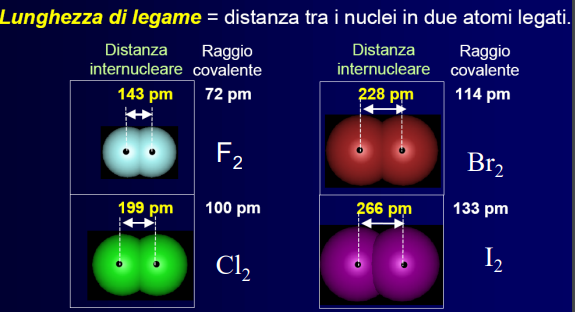
\includegraphics[width=12cm]{immagini/molecole_biatomiche_alogeni.png}
\end{figure}

Tra le varie molecole cambia la dimensione dell'alogeno. Infatti man mano che scendiamo lungo un gruppo si salta di un'unità di numero quantico principale, per cui aumentano dimensioni e lunghezza di legame.

Nel caso delle molecole biatomiche omonucleari si assume che quando si forma il legame chimico i due atomi vadano ad essere in contatto tra loro, per cui dividendo la distanza di legame in due si assegna un raggio (detto atomico o covalente) all'elemento considerato.

\begin{center}
    \begin{tabular}{m{2.7cm}m{2.3cm}m{3cm}m{2.7cm}}
        Legame & \hspace{-0.6cm}Ordine di & \hspace{-1cm}Lunghezza media & \hspace{-0.6cm}Energia media\\
        & \vspace{-0.3cm}\hspace{-0.5cm}Legame & \hspace{-0.9cm}di Legame (pm) & \hspace{-1cm}di legame (kj/mol)\\[0.2ex] 
        \hline
        $\ce{C-O}$ & 1 & 143 & 358\\
        $\ce{C=O}$ & 2 & 123 & 745\\
        $\ce{C#O}$ & 3 & 113 & \hspace{-0.1cm}1070\\
        $\ce{C-C}$ & 1 & 154 & 347\\
        $\ce{C=C}$ & 2 & 134 & 614\\
        $\ce{C#C}$ & 3 & 121 & 839\\
        $\ce{N-N}$ & 1 & 146 & 160\\
        $\ce{N=N}$ & 2 & 122 & 418\\
        $\ce{N#N}$ & 3 & 110 & 945
    \end{tabular}
\end{center}

Per le molecole eteronucleari invece la lunghezza di legame diminuisce all'aumentare dell'O.L.\,: i nuclei sono spinti più vicino dall'attrazione conseguente all'aumento del numero delle coppie elettronice. Al contrario, l'energia di legame aumenta con l'O.L.\,. In generale, più un legame è corto più è forte.

\subsection{Proprietà fisiche dei composti covalenti}
Arrivati a questo punto siamo in grado di descrivere, sulla base della struttura elettronica, le proprietà dei sistemi.

Parliamo dei legami covalenti e dei solidi covalenti in generale. 

I legami covalenti sono molto forti, cioè hanno energie molto consistenti. Quindi forti forze di legame covalente tengono assieme gli atomi in una molecola. Tuttavia, contrariamente ai sistemi ionici, le forze intermolecolari (che è ciò che tiene insieme in un solido le molecole all'interno delle quali vi è un legame covalente) sono deboli. Questo significa che, essendo le forze intermolecolari facili da battere, un composto covalente tipicamente fonde e va in ebollizione facilmente, ossia le loro temperature di fusione ed ebollizione non sono alte come lo erano quelle dei solidi ionici. Ne è un esempio il pentano C$_5$H$_{12}$. Esso è un liquido spesso usato come solvente, il quale bolle sopra i 4° C perché per far bollire questo sistema dobbiamo rompere le interazioni intermolecolari, le quali però sono deboli e quindi facili da rompere.

Ci sono però delle eccezioni, come ad esempio il diamante. Esso è formato da carbonio con coordinazione tetraedrica. È simile alla grafite, solo che nel diamante si ha ibridizzazione $\rm sp^3$, nella grafite $\rm sp^2$, per cui il carbonio grafitico è a strati. Ciò però da un punto di vista termodinamico conferisce maggiore stabilità rispetto al diamante, tant'è che i diamanti nel tempo si trasformano in grafite.

Nel diamante troviamo un reticolo, simile a quello dei solidi ionici, costituito da tetraedri incastonati tra loro. Ciò porta il diamante ad avere il punto di fusione a 3550° C.

\vspace{0.2cm} Un altro esempio è il quarzo, che è la forma cristallina del SiO$_2$ di cui è fatto il vetro, il quale però non è cristallino ma amorfo. La differenza tra vetro e quarzo sta nel fatto che il quarzo ha un reticolo, il vetro no.

Il quarzo ha un punto di ebollizione di 1550° C.

Quindi esistono degli esempi di reticoli covalenti, in cui torniamo al concetto di energia del reticolo, ma nella maggioranza dei casi il reticolo non è presente nei solidi covalenti.

\hspace{0.7cm}\begin{minipage}{0.5 \textwidth}
    \begin{figure}[H]
        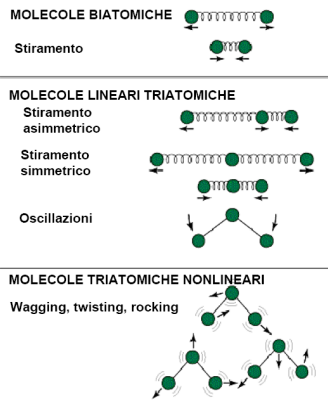
\includegraphics[width=7cm]{immagini/vibrazioni.png}
    \end{figure}
\end{minipage}
\begin{minipage}{0.4 \textwidth}
\vspace{-0.4cm}Va da ricordare che quando si parla di reticoli si parla di posizioni ben precise che si ripetono per traslazione lungo le tre dimensioni. Inoltre tutte le volte che incontriamo un valore di qualche caratteristica, esso è un valore medio, in quanto le molecole vibrano attorno alla distanza di equilibrio. Se poi cresce il numero di atomi, le vibrazioni possono essere simmetriche o asimmetriche e ci possono anche essere deformazioni. dell'angolo dette bending. Ciò vale per molecole lineari, per quelle non lineari si hanno altri movimenti ancora. Quindi ragioniamo sempre su configurazioni di equilibrio ben precise, cioè quelle che hanno la minima energia.
\end{minipage}